% -*- mode: Noweb; noweb-code-mode: perl-mode; tab-width: 4 -*-% ===> this file was generated automatically by noweave --- better not edit it
\documentclass[11pt]{article}
%
%2345678901234567890123456789012345678901234567890123456789012345678901234567890
%        1         2         3         4         5         6         7         8
%
% $Id: SintenicGenePrediction.tex,v 1.3 2001-06-06 19:00:58 jabril Exp $
%
\usepackage{noweb}
\usepackage[a4paper,offset={0pt,0pt},hmargin={2cm,2cm},vmargin={1cm,1cm}]{geometry}
\usepackage{graphics}
\usepackage[dvips]{graphicx}
%% pstricks
\usepackage[dvips]{pstcol}
\usepackage{pstricks}
%\usepackage{pst-node}
%\usepackage{pst-char}
%\usepackage{pst-grad}
%% bibliography
\usepackage{natbib}
%% latex2html
\usepackage{url}
\usepackage{html}     
\usepackage{htmllist} 
%% tables    
%\usepackage{colortbl}
%\usepackage{multirow}
%\usepackage{hhline}
%\usepackage{tabularx}
%\usepackage{dcolumn}
%% seminar
%\usepackage{semcolor,semlayer,semrot,semhelv,sem-page,slidesec}
%% draft watermark
%\usepackage[all,dvips]{draftcopy}
%\draftcopySetGrey{0.9}
%\draftcopyName{CONFIDENTIAL}{100}
%% layout
\usepackage{fancyhdr} % Do not use \usepackage{fancybox} -> TOCs disappear
%\usepackage{lscape}
%\usepackage{rotating}
%\usepackage{multicol}
%% fonts
\usepackage{times}\fontfamily{ptm}\selectfont
\usepackage{t1enc}

% noweb options
\noweboptions{smallcode}
\def\nwendcode{\endtrivlist \endgroup} % relax page breaking scheme
\let\nwdocspar=\par                    %
 
% Colors for gff2ps
\input ColorDefs.tex
% New Commands are defined here
\newcommand{\sctn}[1]{\section{#1}}
\newcommand{\subsctn}[1]{\subsection{#1}}
\newcommand{\subsubsctn}[1]{\subsubsection{#1}}
\newcommand{\desc}[1]{\item[#1] \ \\}

% PSTRICKs definitions
\pslongbox{ExFrame}{\psframebox}
\newcommand{\cln}[1]{\fcolorbox{black}{#1}{\textcolor{#1}{\rule[-.3ex]{1cm}{1ex}}}}
\newpsobject{showgrid}{psgrid}{subgriddiv=0,griddots=1,gridlabels=6pt}
% \pscharpath[fillstyle=solid, fillcolor=verydarkcyan, linecolor=black, linewidth=1pt]{\sffamily\scshape\bfseries\veryHuge #1 }

%%%%% global urls
% \newcommand{\getpsf}[1]{\html{(\htmladdnormallink{Get PostScript file}{./Psfiles/#1})}}   
\def\mtjabril{\htmladdnormallink{\textbf{jabril@imim.es}}{MAILTO:jabril@imim.es}}

% defs
\def\drome{\textit{Drosophila melanogaster}}
\def\dro{\textit{Drosophila}}
\def\dme{\textit{D. melanogaster}}
\def\seq{\texttt{\textbf{X62937}}}
\def\nowf{{\Tt{}SintenicGenePrediction.nw}}
\def\rptm{\textsc{RepeatMasker}}
\def\bl{\textsc{Blast}}
\def\bn{\textsc{blastn}}
\def\bx{\textsc{blastx}}
\def\bp{\textsc{blastp}}
\def\tbn{\textsc{tblastn}}
\def\tbx{\textsc{tblastx}}
\def\ps{\textsc{PostScript}}
\def\gnid{\texttt{geneid}}
\def\gnsc{\texttt{genscan}}
\def\prog{\textsc{sgp}}

% Setting text for footers and headers

\def\tit{\textsc{Sintenic Gene Prediction Tool.- }}
\fancyhead{} % clear all fields
\fancyfoot{} % clear all fields
\fancyhead[RO,LE]{\thepage}
\fancyhead[LO,RE]{\rightmark}
\fancyfoot[LO,LE]{\small\textsl{Guig\`o, Parra, Abril}}
\fancyfoot[RO,RE]{\small\textbf{\today}}
\renewcommand{\headrulewidth}{1pt}
\renewcommand{\footrulewidth}{1pt}

%%%%%%%%%%%%%%%%%%%%%%%%%%%%%%%%%%%%%%%%%%%%%%%%%%%%%%%%%%%%%%%%%%%%%%%%%%%

\begin{document}
\nwfilename{/home/ug/jabril/development/sggp/SintenicGenePrediction.nw}\nwbegindocs{1}\nwdocspar
\thispagestyle{empty}

\begin{titlepage}

\ \vfill
\begin{center}
\textbf{\Huge Sintenic Gene Prediction Tool}\\[5ex]

\textbf{\Large Roderic Guig\`o}\\[1ex]
\textbf{\Large Gen\'{\i}s Parra}\\[1ex]
\textbf{\Large Josep F. Abril}\\[5ex] % \raisebox{0.85ex}{\footnotesize$\,\dag$}\\[0.5ex]

\textbf{\large --- \today ---}\\[10ex]

\begin{abstract}
\begin{center}
\parbox{0.75\linewidth}{
The project main goal is to implement the {\prog} tool in Perl, make its parameters able to get configured through a customization file, and draft a script to automatize fine tunning of the program. We have to include in the distributable package a modified version of {\gnid}. We will need to optimize the {\bl} databases in order to increase query search speed when long subject sequences are given.
} % parbox
\end{center}
\end{abstract}

\vfill

\begin{raggedleft}
\scalebox{0.9 1}{\Large\textsl{\textbf{Genome Informatics Research Lab}}}\\
Grup de Recerca en Infom\`atica Biom\`edica\\
Institut Municipal d'Investigaci\'o M\`edica\\
Universitat Pompeu Fabra\\[2ex]
\raisebox{0.85ex}{\footnotesize$\dag\,$}{\large e-mail: \mtjabril}\\
\end{raggedleft}
\end{center}

\end{titlepage} %'

%%%%%%%%%%%%%%%%%%%% FRONTMATTER

\newpage
\pagenumbering{roman}
\setcounter{page}{1}
\pagestyle{fancy}
% Marks redefinition must go here because pagestyle 
% resets the values to the default ones.
\renewcommand{\sectionmark}[1]{\markboth{}{\thesection.\ #1}}
\renewcommand{\subsectionmark}[1]{\markboth{}{\thesubsection.\ \textsl{#1}}}

\tableofcontents
\listoftables
\listoffigures

\vfill
\begin{center}
{\small$<$ \verb$Id: SintenicGenePrediction.tex,v 1.3 2001-06-06 19:00:58 jabril Exp $$>$ }
\end{center}

%%%%%%%%%%%%%%%%%%%% MAINMATTER

\newpage
\pagenumbering{arabic}
\setcounter{page}{1}

\sctn{Introduction}

\subsctn{On using comparative genomics to improve gene prediction at genomic scale.}

Conservation in the genomic sequence of species at the appropiate
phylogenetic distance may be indicative of conservation of sequence
function.  We investigate here how sequence conservation may be
indicative of coding function, and develop program, SGP-2, which
integrates the results from {\gnid} and {\tbx} to produce gene
predictions when comparing human/mouse sintenic regions.  We set up a
number benchmark data sets, in which we benchmark {\prog} efficiency
and we test it against \textit{ab initio} programs, sequence similarity
based programs, and other hibrid programs.

% How the program works...
\subsctn{Overall algorithm}

Figure~\ref{fig:algo2} describes the approach in {\prog}.  Given two
genomic sequences, we follow the protocol outlined here: 

\begin{enumerate}
\item mask the sequences using {\rptm},
\item run {\tbx} of one sequence agains the other,
\item ``project'' the similarity regions onto each sequence,
\item  run {\gnid} on each sequence with the projected similarity regions.
\end{enumerate}

\begin{figure}
\begin{center}
\framebox{
\includegraphics[width=0.85\linewidth, trim= 10 10 20 10, clip]{./psfigures/algo2.ps}
}
\end{center}
\caption{\label{fig:algo2} Schemma of the homology-based gene-prediction used in this project.}
\end{figure}

\sctn{The parameters file}

\sctn{Parameter optimization}

%%%%%%%%%%%%%%%%%%%%%%%%%%%%%%%%%%%
\begin{comment}
\end{comment}
%%%%%%%%%%%%%%%%%%%%%%%%%%%%%%%%%%%

%%%%%%%%%%%%%%%%%%%% BACKMATTER

% \newpage
% 
% \bibliographystyle{apalike}
% \bibliography{/home1/rguigo/docs/biblio/References}

\newpage
\appendix

\sctn{Sintenic Gene Prediction tool}

Our initial program outline (our root chunk) looks like:\\[1ex]

\nwenddocs{}\nwbegincode{2}\sublabel{NWSinw-SGP8-1}\nwmargintag{{\nwtagstyle{}\subpageref{NWSinw-SGP8-1}}}\moddef{SGP TOOL~{\nwtagstyle{}\subpageref{NWSinw-SGP8-1}}}\endmoddef\nwstartdeflinemarkup\nwenddeflinemarkup
\LA{}PERL shebang~{\nwtagstyle{}\subpageref{NWSinw-PERC-1}}\RA{}
\LA{}SGP Copyleft~{\nwtagstyle{}\subpageref{NWSinw-SGPC-1}}\RA{}

#### MODULES ####

\LA{}Use Modules - SGP~{\nwtagstyle{}\subpageref{NWSinw-UseH-1}}\RA{} 

#### CONSTANTS DEFINITION ####

\LA{}Constant definition - SGP~{\nwtagstyle{}\subpageref{NWSinw-ConP-1}}\RA{}

#### GLOBAL VARIABLES ####

\LA{}Global Vars - SGP~{\nwtagstyle{}\subpageref{NWSinw-GloH-1}}\RA{}

#### MAIN LOOP ####

    \LA{}Main Loop - SGP~{\nwtagstyle{}\subpageref{NWSinw-MaiF-1}}\RA{}

##### SUBS #####

\LA{}Main Routines - SGP~{\nwtagstyle{}\subpageref{NWSinw-MaiJ-1}}\RA{}

#### EOF ####

\LA{}POD man page - SGP~{\nwtagstyle{}\subpageref{NWSinw-PODI-1}}\RA{}
\nwnotused{SGP TOOL}\nwendcode{}\nwbegindocs{3}% 


A short description, followed by authors list and the GNU-GPL, appears at the begining of the code.

\nwenddocs{}\nwbegincode{4}\sublabel{NWSinw-SGPC-1}\nwmargintag{{\nwtagstyle{}\subpageref{NWSinw-SGPC-1}}}\moddef{SGP Copyleft~{\nwtagstyle{}\subpageref{NWSinw-SGPC-1}}}\endmoddef\nwstartdeflinemarkup\nwusesondefline{\\{NWSinw-SGP8-1}}\nwenddeflinemarkup
######################################################################
#                               SGP                                  #
######################################################################
#
#     Sinteny based Gene Prediction tool.
#
#     Copyright (C) 2001 - Josep Francesc ABRIL FERRANDO
#                                   Genis PARRA FARRE
#                                 Roderic GUIGO SERRA
\LA{}Copyleft~{\nwtagstyle{}\subpageref{NWSinw-Cop8-1}}\RA{}
\nwused{\\{NWSinw-SGP8-1}}\nwendcode{}\nwbegindocs{5}\nwdocspar

\subsctn{Main code chunks}

\nwenddocs{}\nwbegincode{6}\sublabel{NWSinw-UseH-1}\nwmargintag{{\nwtagstyle{}\subpageref{NWSinw-UseH-1}}}\moddef{Use Modules - SGP~{\nwtagstyle{}\subpageref{NWSinw-UseH-1}}}\endmoddef\nwstartdeflinemarkup\nwusesondefline{\\{NWSinw-SGP8-1}}\nwenddeflinemarkup
\LA{}Use Modules - Benchmark~{\nwtagstyle{}\subpageref{NWSinw-UseN-1}}\RA{}
\LA{}Use Modules - Dumper~{\nwtagstyle{}\subpageref{NWSinw-UseK-1}}\RA{}
\nwused{\\{NWSinw-SGP8-1}}\nwendcode{}\nwbegindocs{7}\nwdocspar

\nwenddocs{}\nwbegincode{8}\sublabel{NWSinw-ConP-1}\nwmargintag{{\nwtagstyle{}\subpageref{NWSinw-ConP-1}}}\moddef{Constant definition - SGP~{\nwtagstyle{}\subpageref{NWSinw-ConP-1}}}\endmoddef\nwstartdeflinemarkup\nwusesondefline{\\{NWSinw-SGP8-1}}\nwenddeflinemarkup
my $PROGRAM = "SGP";
my @tmp_ver = split / +/, 
    ': $Id: SintenicGenePrediction.tex,v 1.3 2001-06-06 19:00:58 jabril Exp $ :';
my $VERSION = "v$tmp_ver[3] [@tmp_ver[4,5,7]]";
\LA{}Global Constants - Boolean~{\nwtagstyle{}\subpageref{NWSinw-GloQ-1}}\RA{}
\LA{}Global Constants - STDERR~{\nwtagstyle{}\subpageref{NWSinw-GloP-1}}\RA{}
\nwused{\\{NWSinw-SGP8-1}}\nwendcode{}\nwbegindocs{9}\nwdocspar

\nwenddocs{}\nwbegincode{10}\sublabel{NWSinw-GloH-1}\nwmargintag{{\nwtagstyle{}\subpageref{NWSinw-GloH-1}}}\moddef{Global Vars - SGP~{\nwtagstyle{}\subpageref{NWSinw-GloH-1}}}\endmoddef\nwstartdeflinemarkup\nwusesondefline{\\{NWSinw-SGP8-1}}\nwenddeflinemarkup
\LA{}Global Vars - User and Date~{\nwtagstyle{}\subpageref{NWSinw-GloR-1}}\RA{}
\LA{}Global Vars - Counter~{\nwtagstyle{}\subpageref{NWSinw-GloL-1}}\RA{}
\LA{}SGP: Global Vars - STDERR~{\nwtagstyle{}\subpageref{NWSinw-SGPP-1}}\RA{}
\nwused{\\{NWSinw-SGP8-1}}\nwendcode{}\nwbegindocs{11}\nwdocspar

\nwenddocs{}\nwbegincode{12}\sublabel{NWSinw-MaiF-1}\nwmargintag{{\nwtagstyle{}\subpageref{NWSinw-MaiF-1}}}\moddef{Main Loop - SGP~{\nwtagstyle{}\subpageref{NWSinw-MaiF-1}}}\endmoddef\nwstartdeflinemarkup\nwusesondefline{\\{NWSinw-SGP8-1}}\nwenddeflinemarkup
&report('START_JOB');
# get options
&Which_Options();
# parameters for
&read_parameter_file();
#
&report('JOB_DONE',&timing($T));
exit(0);
\nwused{\\{NWSinw-SGP8-1}}\nwidentuses{\\{{\nwixident{{\&}read{\_}parameter{\_}file}}{:amread:unparameter:unfile}}\\{{\nwixident{{\&}report}}{:amreport}}\\{{\nwixident{{\$}T}}{:doT}}\\{{\nwixident{{\&}timing}}{:amtiming}}\\{{\nwixident{{\&}Which{\_}Options}}{:amWhich:unOptions}}}\nwindexuse{\nwixident{{\&}read{\_}parameter{\_}file}}{:amread:unparameter:unfile}{NWSinw-MaiF-1}\nwindexuse{\nwixident{{\&}report}}{:amreport}{NWSinw-MaiF-1}\nwindexuse{\nwixident{{\$}T}}{:doT}{NWSinw-MaiF-1}\nwindexuse{\nwixident{{\&}timing}}{:amtiming}{NWSinw-MaiF-1}\nwindexuse{\nwixident{{\&}Which{\_}Options}}{:amWhich:unOptions}{NWSinw-MaiF-1}\nwendcode{}\nwbegindocs{13}\nwdocspar

\nwenddocs{}\nwbegincode{14}\sublabel{NWSinw-SGPL-1}\nwmargintag{{\nwtagstyle{}\subpageref{NWSinw-SGPL-1}}}\moddef{SGP: runtime messages~{\nwtagstyle{}\subpageref{NWSinw-SGPL-1}}}\endmoddef\nwstartdeflinemarkup\nwusesondefline{\\{NWSinw-SGPP-2}}\nwenddeflinemarkup
START_JOB => "$line$s    RUNNING: $PROGRAM\\n".
                  "$s       USER: $USER\\n".
                  "$s       DATE: $DATE\\n$line$r",
JOB_DONE  => "$line$s  TOTAL TIME SPENT --> \\%s\\n$line",
HEADER    => "$line\\%s$line",
TIMING    => "$r$s  \\%s ...... DONE\\n$s  Time Spent: \\%s$r",
\nwused{\\{NWSinw-SGPP-2}}\nwidentuses{\\{{\nwixident{{\$}DATE}}{:doDATE}}\\{{\nwixident{{\$}USER}}{:doUSER}}}\nwindexuse{\nwixident{{\$}DATE}}{:doDATE}{NWSinw-SGPL-1}\nwindexuse{\nwixident{{\$}USER}}{:doUSER}{NWSinw-SGPL-1}\nwendcode{}\nwbegindocs{15}\nwdocspar

\nwenddocs{}\nwbegincode{16}\sublabel{NWSinw-ComP-1}\nwmargintag{{\nwtagstyle{}\subpageref{NWSinw-ComP-1}}}\moddef{Common PERL subs - STDERR~{\nwtagstyle{}\subpageref{NWSinw-ComP-1}}}\endmoddef\nwstartdeflinemarkup\nwusesondefline{\\{NWSinw-MaiJ-1}}\nwprevnextdefs{\relax}{NWSinw-ComP-2}\nwenddeflinemarkup
sub prt_header() \{
    my $msg = $_[0];
    my $l = $term_width - (2 * length($s));
    $msg = &fill_mid($msg,$l,' ');
    &report('HEADER',$msg);
\} # prt_header
\nwindexdefn{\nwixident{{\&}prt{\_}header}}{:amprt:unheader}{NWSinw-ComP-1}\eatline
\nwalsodefined{\\{NWSinw-ComP-2}\\{NWSinw-ComP-3}}\nwused{\\{NWSinw-MaiJ-1}}\nwidentdefs{\\{{\nwixident{{\&}prt{\_}header}}{:amprt:unheader}}}\nwidentuses{\\{{\nwixident{{\&}fill{\_}mid}}{:amfill:unmid}}\\{{\nwixident{{\&}report}}{:amreport}}}\nwindexuse{\nwixident{{\&}fill{\_}mid}}{:amfill:unmid}{NWSinw-ComP-1}\nwindexuse{\nwixident{{\&}report}}{:amreport}{NWSinw-ComP-1}\nwendcode{}\nwbegindocs{17}\nwdocspar
\nwenddocs{}\nwbegincode{18}\sublabel{NWSinw-MaiJ-1}\nwmargintag{{\nwtagstyle{}\subpageref{NWSinw-MaiJ-1}}}\moddef{Main Routines - SGP~{\nwtagstyle{}\subpageref{NWSinw-MaiJ-1}}}\endmoddef\nwstartdeflinemarkup\nwusesondefline{\\{NWSinw-SGP8-1}}\nwenddeflinemarkup
\LA{}SGP: parsing command-line~{\nwtagstyle{}\subpageref{NWSinw-SGPP.2-1}}\RA{}
\LA{}SGP: parsing parameters file~{\nwtagstyle{}\subpageref{NWSinw-SGPS-1}}\RA{}
\LA{}SGP: run blast~{\nwtagstyle{}\subpageref{NWSinw-SGPE-1}}\RA{}
\LA{}SGP: extract HSPs~{\nwtagstyle{}\subpageref{NWSinw-SGPH-1}}\RA{}
\LA{}SGP: run geneid~{\nwtagstyle{}\subpageref{NWSinw-SGPF-1}}\RA{}
\LA{}SGP: graphical output~{\nwtagstyle{}\subpageref{NWSinw-SGPL.2-1}}\RA{}
\LA{}Common PERL subs - Check sys command~{\nwtagstyle{}\subpageref{NWSinw-Coma-1}}\RA{}
\LA{}Common PERL subs - Min Max~{\nwtagstyle{}\subpageref{NWSinw-ComQ-1}}\RA{}
\LA{}Common PERL subs - Text fill~{\nwtagstyle{}\subpageref{NWSinw-ComS.2-1}}\RA{}
\LA{}Common PERL subs - Counter~{\nwtagstyle{}\subpageref{NWSinw-ComQ.2-1}}\RA{}
\LA{}Common PERL subs - STDERR~{\nwtagstyle{}\subpageref{NWSinw-ComP-1}}\RA{}
\nwused{\\{NWSinw-SGP8-1}}\nwendcode{}\nwbegindocs{19}\nwdocspar

\subsctn{Reporting to {\Tt{}STDERR}}

\nwenddocs{}\nwbegincode{20}\sublabel{NWSinw-GloP-1}\nwmargintag{{\nwtagstyle{}\subpageref{NWSinw-GloP-1}}}\moddef{Global Constants - STDERR~{\nwtagstyle{}\subpageref{NWSinw-GloP-1}}}\endmoddef\nwstartdeflinemarkup\nwusesondefline{\\{NWSinw-ConP-1}}\nwenddeflinemarkup
my $term_width = 60;
my $line = ("#" x $term_width)."\\n";
my ($s,$r) = ("###","###\\n");
my $Error = "\\<\\<\\<  ERROR  \\>\\>\\> "; # scaped symbols to avoid 
my $Warn  = "\\<\\<\\< WARNING \\>\\>\\> "; #     problems with noweb
my $spw   = "\\<\\<\\<         \\>\\>\\> ";
my $spl   = "\\<\\<\\<\\-\\-\\-\\-\\-\\-\\-\\-\\-\\>\\>\\>\\n";
\nwused{\\{NWSinw-ConP-1}}\nwendcode{}\nwbegindocs{21}\nwdocspar

\nwenddocs{}\nwbegincode{22}\sublabel{NWSinw-SGPB-1}\nwmargintag{{\nwtagstyle{}\subpageref{NWSinw-SGPB-1}}}\moddef{SGP: errors~{\nwtagstyle{}\subpageref{NWSinw-SGPB-1}}}\endmoddef\nwstartdeflinemarkup\nwusesondefline{\\{NWSinw-SGPP-1}}\nwenddeflinemarkup
\nwused{\\{NWSinw-SGPP-1}}\nwendcode{}\nwbegindocs{23}\nwdocspar
\nwenddocs{}\nwbegincode{24}\sublabel{NWSinw-SGPD-1}\nwmargintag{{\nwtagstyle{}\subpageref{NWSinw-SGPD-1}}}\moddef{SGP: messages~{\nwtagstyle{}\subpageref{NWSinw-SGPD-1}}}\endmoddef\nwstartdeflinemarkup\nwusesondefline{\\{NWSinw-SGPP-2}}\nwenddeflinemarkup
\nwused{\\{NWSinw-SGPP-2}}\nwendcode{}\nwbegindocs{25}\nwdocspar

\nwenddocs{}\nwbegincode{26}\sublabel{NWSinw-SGPP-1}\nwmargintag{{\nwtagstyle{}\subpageref{NWSinw-SGPP-1}}}\moddef{SGP: Global Vars - STDERR~{\nwtagstyle{}\subpageref{NWSinw-SGPP-1}}}\endmoddef\nwstartdeflinemarkup\nwusesondefline{\\{NWSinw-GloH-1}}\nwprevnextdefs{\relax}{NWSinw-SGPP-2}\nwenddeflinemarkup
#
# Error/Warning Message List
my %ErrorList = (
                 \LA{}SGP: errors~{\nwtagstyle{}\subpageref{NWSinw-SGPB-1}}\RA{}
                 \LA{}SGP: commandline warnings~{\nwtagstyle{}\subpageref{NWSinw-SGPP.3-1}}\RA{}
                 );
\nwalsodefined{\\{NWSinw-SGPP-2}}\nwused{\\{NWSinw-GloH-1}}\nwendcode{}\nwbegindocs{27}\nwdocspar

\nwenddocs{}\nwbegincode{28}\sublabel{NWSinw-SGPP-2}\nwmargintag{{\nwtagstyle{}\subpageref{NWSinw-SGPP-2}}}\moddef{SGP: Global Vars - STDERR~{\nwtagstyle{}\subpageref{NWSinw-SGPP-1}}}\plusendmoddef\nwstartdeflinemarkup\nwusesondefline{\\{NWSinw-GloH-1}}\nwprevnextdefs{NWSinw-SGPP-1}{\relax}\nwenddeflinemarkup
#
# Verbose Message List
my %MessageList = (
                   \LA{}SGP: messages~{\nwtagstyle{}\subpageref{NWSinw-SGPD-1}}\RA{}
                   \LA{}SGP: runtime messages~{\nwtagstyle{}\subpageref{NWSinw-SGPL-1}}\RA{}
                   );
\nwused{\\{NWSinw-GloH-1}}\nwendcode{}\nwbegindocs{29}\nwdocspar

\subsctn{Removing temporary files}

In such cases that we stop the program execution or it hangs up, we have to clean temporary path from any temporary files we have created.

\nwenddocs{}\nwbegincode{30}\sublabel{NWSinw-traK-1}\nwmargintag{{\nwtagstyle{}\subpageref{NWSinw-traK-1}}}\moddef{trap temporary files~{\nwtagstyle{}\subpageref{NWSinw-traK-1}}}\endmoddef\nwstartdeflinemarkup\nwenddeflinemarkup
$SIG\{INT\}  = \\&trap_signals;
$SIG\{QUIT\} = \\&trap_signals;
$SIG\{TERM\} = \\&trap_signals;
$SIG\{CHLD\} = 'IGNORE';
sub trap_signals() \{
    # opendir(TDIR, $TMP) or &go_to_die("Can't open directory $TMP: $!");
    # while (defined(my $file = readdir(TDIR)))
    &clean_tmp();
    &go_to_die("WARNING !!! $PROGRAM has been stopped by user.");
\}
\nwnotused{trap temporary files}\nwendcode{}\nwbegindocs{31}%$

The following signals are trapped by our signal handler routine (to be precise, when assigning to {\Tt{}{\$}SIG} the call by reference to that routine): %$
\begin{itemize}\setlength{\itemsep}{-0.5ex}
\item {\Tt{}SIGINT} is normally triggered by Ctrl-C, requesting that a process interrupt what it's doing.%'
\item {\Tt{}SIGQUIT} is also generated by a terminal, usually Ctrl-$\backslash$, generating a core dump.
\item {\Tt{}SIGTERM} is sent by {\Tt{}kill} shell command when no signal name is explicitly given (think of it as a polite request for a process to die). 
\end{itemize}

\subsctn{Parsing command-line options}

\nwenddocs{}\nwbegincode{32}\sublabel{NWSinw-decC-1}\nwmargintag{{\nwtagstyle{}\subpageref{NWSinw-decC-1}}}\moddef{declare uses~{\nwtagstyle{}\subpageref{NWSinw-decC-1}}}\endmoddef\nwstartdeflinemarkup\nwprevnextdefs{\relax}{NWSinw-decC-2}\nwenddeflinemarkup
use Getopt::Long;
Getopt::Long::Configure qw/ bundling pass_through /;
\nwalsodefined{\\{NWSinw-decC-2}\\{NWSinw-decC-3}}\nwnotused{declare uses}\nwendcode{}\nwbegindocs{33}\nwdocspar

\begin{description}\setlength{\itemsep}{-0.5ex}
\desc{{\Tt{}use\ Getopt::Long;}} This module implements an extended getopt function called {\Tt{}GetOptions()}. This function adheres to the POSIX syntax for command line options, with GNU extensions. In general, this means that options having long names instead of single letters are introduced with a double dash "-\/-". A double dash on itself signals end of the options list and start of the input 'files'.

\desc{{\Tt{}Getopt::Long::Configure\ qw(\ bundling\ pass{\_}through\ );}} {\Tt{}GetOptions} can be configured by calling subroutine {\Tt{}Getopt::Long::Configure}. This subroutine takes a list of quoted strings, each specifying a configuration option to be set. Options can be reset by prefixing with '{\Tt{}no{\_}}'. 

 \begin{description}\setlength{\itemsep}{-0.5ex}
 \desc{{\Tt{}bundling}} Support for bundling of command line options, as was the case with the more traditional single-letter approach (introduced with a single dash "-"), is provided but not enabled by default. 

 \desc{{\Tt{}pass{\_}through}} Unknown options are passed through in {\Tt{}@ARGV} instead of being flagged as errors. This makes it possible to write wrapper scripts that process only part of the user supplied options, and passes the remaining options to some other program.
 \end{description}
\end{description}

\nwenddocs{}\nwbegincode{34}\sublabel{NWSinw-decH-1}\nwmargintag{{\nwtagstyle{}\subpageref{NWSinw-decH-1}}}\moddef{declare variables~{\nwtagstyle{}\subpageref{NWSinw-decH-1}}}\endmoddef\nwstartdeflinemarkup\nwprevnextdefs{\relax}{NWSinw-decH-2}\nwenddeflinemarkup
# GetOptions Variables
my ( $Seq1, $Seq2, $geneid_opt, $geneid_param, 
     $blast_opt, $score_cutoff, $shrink, $tbx,
     $hsp, $ofn, $ps_output, $savefiles_flg, $verbose_flg, $help_flg
     ) = ( undef, undef, undef, undef, undef, undef,
           undef, undef, undef, undef, undef, 0, 0, 0 );
\nwalsodefined{\\{NWSinw-decH-2}\\{NWSinw-decH-3}}\nwnotused{declare variables}\nwendcode{}\nwbegindocs{35}%

Those variables will receive the values passed from command-line options in {\Tt{}Which{\_}Options()} function. We set them as {\Tt{}undef} to check after {\Tt{}Which{\_}Options()} if they have received any value (testing them with perl built-in {\Tt{}defined()} function).

\nwenddocs{}\nwbegincode{36}\sublabel{NWSinw-SGPP.2-1}\nwmargintag{{\nwtagstyle{}\subpageref{NWSinw-SGPP.2-1}}}\moddef{SGP: parsing command-line~{\nwtagstyle{}\subpageref{NWSinw-SGPP.2-1}}}\endmoddef\nwstartdeflinemarkup\nwusesondefline{\\{NWSinw-MaiJ-1}}\nwenddeflinemarkup
# Parsing command-line options and processing its parameters.
\LA{}getopts subs~{\nwtagstyle{}\subpageref{NWSinw-getC-1}}\RA{}
sub Which_Options() \{
    $SIG\{__WARN__\} = sub \{ &warn('UNKNOWN_CL_OPTION',$_[0]) \};
    GetOptions( 
                "1=s"      => \\$Seq1         , # seqfile_1
                "2=s"      => \\$Seq2         , # seqfile_2
                "g=s"      => \\$geneid_opt   , # geneid options      
                "P=s"      => \\$geneid_param , # geneid parameter file 
                "o=s"      => \\$blast_opt    , # tblastx options 
                "c=f"      => \\$score_cutoff , # tblastx score cutoff
                "s=f"      => \\$shrink       , # shrink hsp's by
                "t=s"      => \\$tbx          , # read tblastx from file
                "f=s"      => \\$hsp          , # read HSP files in directory
                "k=s"      => \\$ofn          , # intermediate filename
                "p=s"      => \\$ps_output    , # postscript output 
                "v"        => \\$verbose_flg  , # verbose    
                "h|help|?" => \\$help_flg     , # print help
                ) || (&warn('CMD_LINE_ERROR'), exit(1));
    $SIG\{__WARN__\} = 'DEFAULT';
    &prt_Help if $help_flg;
    &prt_Header("Processsing Command-Line Options") if $verbose_flg;
    \LA{}set flags-vars~{\nwtagstyle{}\subpageref{NWSinw-setE-1}}\RA{}
\} # sub Which_Options
\nwindexdefn{\nwixident{{\&}Which{\_}Options}}{:amWhich:unOptions}{NWSinw-SGPP.2-1}\eatline
\nwused{\\{NWSinw-MaiJ-1}}\nwidentdefs{\\{{\nwixident{{\&}Which{\_}Options}}{:amWhich:unOptions}}}\nwidentuses{\\{{\nwixident{{\&}warn}}{:amwarn}}}\nwindexuse{\nwixident{{\&}warn}}{:amwarn}{NWSinw-SGPP.2-1}\nwendcode{}\nwbegindocs{37}%$

\nwenddocs{}\nwbegincode{38}\sublabel{NWSinw-SGPP.3-1}\nwmargintag{{\nwtagstyle{}\subpageref{NWSinw-SGPP.3-1}}}\moddef{SGP: commandline warnings~{\nwtagstyle{}\subpageref{NWSinw-SGPP.3-1}}}\endmoddef\nwstartdeflinemarkup\nwusesondefline{\\{NWSinw-SGPP-1}}\nwenddeflinemarkup
UNKNOWN_CL_OPTION => "!!! Error trapped while processing command-line:\\n",
CMD_LINE_ERROR => "!!! Please, check your command-line options!!!\\n",
\nwused{\\{NWSinw-SGPP-1}}\nwendcode{}\nwbegindocs{39}\nwdocspar
 
In {\Tt{}GetOptions()} function, sufixing an option with '=s' implies that it will require a mandatory string parameter, with '=f' the option must be provided with a real number. The following variables need a filename: {\Tt{}{\$}geneid{\_}param} {\Tt{}{\$}tbx} {\Tt{}{\$}hsp} {\Tt{}{\$}ofn} {\Tt{}{\$}ps{\_}output}.%$

\begin{comment}
\todo{get options}{
 \item {\Tt{}{\$}score{\_}cutoff} and {\Tt{}{\$}shrink} still not used. 
 \item Define better how the paths/filenames are passed through those options. Remember that these variables will be defined by giving a path, but some need a prefix.
}
\end{comment}
 
\nwenddocs{}\nwbegincode{40}\sublabel{NWSinw-getC-1}\nwmargintag{{\nwtagstyle{}\subpageref{NWSinw-getC-1}}}\moddef{getopts subs~{\nwtagstyle{}\subpageref{NWSinw-getC-1}}}\endmoddef\nwstartdeflinemarkup\nwusesondefline{\\{NWSinw-SGPP.2-1}}\nwenddeflinemarkup
# Checking input sequence files
sub exists_file() \{
    my @files = @_;
    my ($n, $r) = (' ', 0);
    foreach $n (@files) \{
        $r++ if (-e "$n");
    \};
    return $r;
\}
sub check_fasta_format() \{
    my $file = $_[0];
    my ($n, $c) = (undef, 0);
    open(TMP,"< $file");
    while (<TMP>) \{
        next unless /^>/;
        />(\\S+)\\b/ && do \{
            $n = $1;
            $c++;
            next unless $c>1;
        \};
        &go_to_die("FATAL ERROR !!! Multiple locus names found.\\n  File \\'$file\\' must contain only one sequence definition.\\n");
    \}
    &go_to_die("FATAL ERROR !!! There is no '>' line, locus name not found.\\n  Please, verify your fasta file \\'$file\\'\\n") unless defined($n);
    return $n;
\}
\nwindexdefn{\nwixident{{\&}exists{\_}file}}{:amexists:unfile}{NWSinw-getC-1}\nwindexdefn{\nwixident{{\&}check{\_}fasta{\_}format}}{:amcheck:unfasta:unformat}{NWSinw-getC-1}\eatline
\nwused{\\{NWSinw-SGPP.2-1}}\nwidentdefs{\\{{\nwixident{{\&}check{\_}fasta{\_}format}}{:amcheck:unfasta:unformat}}\\{{\nwixident{{\&}exists{\_}file}}{:amexists:unfile}}}\nwidentuses{\\{{\nwixident{{\$}c}}{:doc}}\\{{\nwixident{{\$}n}}{:don}}}\nwindexuse{\nwixident{{\$}c}}{:doc}{NWSinw-getC-1}\nwindexuse{\nwixident{{\$}n}}{:don}{NWSinw-getC-1}\nwendcode{}\nwbegindocs{41}%$

{\Tt{}exists{\_}file()} : Given a list of filenames, this function returns how many among them does exist.

{\Tt{}check{\_}fasta{\_}format()} : For a given file, returns the \textit{locus} name if file is in {\Tt{}fasta} format, else program dies.

\nwenddocs{}\nwbegincode{42}\sublabel{NWSinw-decC-2}\nwmargintag{{\nwtagstyle{}\subpageref{NWSinw-decC-2}}}\moddef{declare uses~{\nwtagstyle{}\subpageref{NWSinw-decC-1}}}\plusendmoddef\nwstartdeflinemarkup\nwprevnextdefs{NWSinw-decC-1}{NWSinw-decC-3}\nwenddeflinemarkup
use File::Basename;
\nwendcode{}\nwbegindocs{43}\nwdocspar

This standard module contains routines to split up a filename. {\Tt{}basename} is provided for programmer compatibility with the same name \textsc{Unix} shell command.

\nwenddocs{}\nwbegincode{44}\sublabel{NWSinw-decH-2}\nwmargintag{{\nwtagstyle{}\subpageref{NWSinw-decH-2}}}\moddef{declare variables~{\nwtagstyle{}\subpageref{NWSinw-decH-1}}}\plusendmoddef\nwstartdeflinemarkup\nwprevnextdefs{NWSinw-decH-1}{NWSinw-decH-3}\nwenddeflinemarkup
# sequence files
my ($Seq1_Name, $Seq2_Name, $Loc1, $Loc2, $SGPtmp1, $SGPtmp2, $SGPtmpG);
\nwindexdefn{\nwixident{{\$}Seq1{\_}Name}}{:doSeq1:unName}{NWSinw-decH-2}\nwindexdefn{\nwixident{{\$}Seq2{\_}Name}}{:doSeq2:unName}{NWSinw-decH-2}\nwindexdefn{\nwixident{{\$}Loc1}}{:doLoc1}{NWSinw-decH-2}\nwindexdefn{\nwixident{{\$}Loc2}}{:doLoc2}{NWSinw-decH-2}\nwindexdefn{\nwixident{{\$}SGPtmp1}}{:doSGPtmp1}{NWSinw-decH-2}\nwindexdefn{\nwixident{{\$}SGPtmp2}}{:doSGPtmp2}{NWSinw-decH-2}\nwindexdefn{\nwixident{{\$}SGPtmpG}}{:doSGPtmpG}{NWSinw-decH-2}\eatline
\nwidentdefs{\\{{\nwixident{{\$}Loc1}}{:doLoc1}}\\{{\nwixident{{\$}Loc2}}{:doLoc2}}\\{{\nwixident{{\$}Seq1{\_}Name}}{:doSeq1:unName}}\\{{\nwixident{{\$}Seq2{\_}Name}}{:doSeq2:unName}}\\{{\nwixident{{\$}SGPtmp1}}{:doSGPtmp1}}\\{{\nwixident{{\$}SGPtmp2}}{:doSGPtmp2}}\\{{\nwixident{{\$}SGPtmpG}}{:doSGPtmpG}}}\nwendcode{}\nwbegindocs{45}\nwdocspar
\nwenddocs{}\nwbegincode{46}\sublabel{NWSinw-setE-1}\nwmargintag{{\nwtagstyle{}\subpageref{NWSinw-setE-1}}}\moddef{set flags-vars~{\nwtagstyle{}\subpageref{NWSinw-setE-1}}}\endmoddef\nwstartdeflinemarkup\nwusesondefline{\\{NWSinw-SGPP.2-1}}\nwprevnextdefs{\relax}{NWSinw-setE-2}\nwenddeflinemarkup
# do seq files exists
my $file_number = &exists_file($Seq1, $Seq2);
&go_to_die("FATAL ERROR!!! Two sequences are needed (-1 and -2 options are mandatory).\\n")
    unless $file_number == 2; 
# extract basenames
$Seq1_Name = basename($Seq1);
$Seq2_Name = basename($Seq2);
# check if files are provided in fasta format and get locus names
$Loc1 = &check_fasta_format($Seq1);
$Loc2 = &check_fasta_format($Seq2);
&go_to_die("FATAL ERROR!!! Locus1($Loc1) have the same name as Locus2($Loc2).\\n  Sequences \\'$Seq1_Name\\' and \\'$Seq2_Name\\' must have different locus names.\\n")
    if $Loc1 eq $Loc2;
# tmpfiles prefix
$SGPtmp1 = "$SGPTMP.$Seq1_Name";
$SGPtmp2 = "$SGPTMP.$Seq2_Name";
$SGPtmpG = "$SGPTMP.$\{Loc1\}_$\{Loc2\}"; 
\nwalsodefined{\\{NWSinw-setE-2}}\nwused{\\{NWSinw-SGPP.2-1}}\nwidentuses{\\{{\nwixident{{\&}check{\_}fasta{\_}format}}{:amcheck:unfasta:unformat}}\\{{\nwixident{{\&}exists{\_}file}}{:amexists:unfile}}\\{{\nwixident{{\$}Loc1}}{:doLoc1}}\\{{\nwixident{{\$}Loc2}}{:doLoc2}}\\{{\nwixident{{\$}Seq1{\_}Name}}{:doSeq1:unName}}\\{{\nwixident{{\$}Seq2{\_}Name}}{:doSeq2:unName}}\\{{\nwixident{{\$}SGPtmp1}}{:doSGPtmp1}}\\{{\nwixident{{\$}SGPtmp2}}{:doSGPtmp2}}\\{{\nwixident{{\$}SGPtmpG}}{:doSGPtmpG}}}\nwindexuse{\nwixident{{\&}check{\_}fasta{\_}format}}{:amcheck:unfasta:unformat}{NWSinw-setE-1}\nwindexuse{\nwixident{{\&}exists{\_}file}}{:amexists:unfile}{NWSinw-setE-1}\nwindexuse{\nwixident{{\$}Loc1}}{:doLoc1}{NWSinw-setE-1}\nwindexuse{\nwixident{{\$}Loc2}}{:doLoc2}{NWSinw-setE-1}\nwindexuse{\nwixident{{\$}Seq1{\_}Name}}{:doSeq1:unName}{NWSinw-setE-1}\nwindexuse{\nwixident{{\$}Seq2{\_}Name}}{:doSeq2:unName}{NWSinw-setE-1}\nwindexuse{\nwixident{{\$}SGPtmp1}}{:doSGPtmp1}{NWSinw-setE-1}\nwindexuse{\nwixident{{\$}SGPtmp2}}{:doSGPtmp2}{NWSinw-setE-1}\nwindexuse{\nwixident{{\$}SGPtmpG}}{:doSGPtmpG}{NWSinw-setE-1}\nwendcode{}\nwbegindocs{47}\nwdocspar

We check here whether the user provided two sequences or not, either they are given in fasta format. We extract locus names and build some base filenames from which we can derive, when needed, several temporary output filenames.

\nwenddocs{}\nwbegincode{48}\sublabel{NWSinw-decH-3}\nwmargintag{{\nwtagstyle{}\subpageref{NWSinw-decH-3}}}\moddef{declare variables~{\nwtagstyle{}\subpageref{NWSinw-decH-1}}}\plusendmoddef\nwstartdeflinemarkup\nwprevnextdefs{NWSinw-decH-2}{\relax}\nwenddeflinemarkup
# file flags
my ($blast_flg, $hsps_flg, $geneid_flg, $plots_flg) = (1, 1, 1, 1);
\nwindexdefn{\nwixident{{\$}blast{\_}flg}}{:doblast:unflg}{NWSinw-decH-3}\nwindexdefn{\nwixident{{\$}hsps{\_}flg}}{:dohsps:unflg}{NWSinw-decH-3}\nwindexdefn{\nwixident{{\$}geneid{\_}flg}}{:dogeneid:unflg}{NWSinw-decH-3}\nwindexdefn{\nwixident{{\$}plots{\_}flg}}{:doplots:unflg}{NWSinw-decH-3}\eatline
\nwidentdefs{\\{{\nwixident{{\$}blast{\_}flg}}{:doblast:unflg}}\\{{\nwixident{{\$}geneid{\_}flg}}{:dogeneid:unflg}}\\{{\nwixident{{\$}hsps{\_}flg}}{:dohsps:unflg}}\\{{\nwixident{{\$}plots{\_}flg}}{:doplots:unflg}}}\nwendcode{}\nwbegindocs{49}\nwdocspar
We initialize those flag variables to '1' in order to get, by default, into all the main subroutines called from main loop. They will be modified when {\Tt{}Which{\_}Options()} function resets some of the option variables. 

\nwenddocs{}\nwbegincode{50}\sublabel{NWSinw-decC-3}\nwmargintag{{\nwtagstyle{}\subpageref{NWSinw-decC-3}}}\moddef{declare uses~{\nwtagstyle{}\subpageref{NWSinw-decC-1}}}\plusendmoddef\nwstartdeflinemarkup\nwprevnextdefs{NWSinw-decC-2}{\relax}\nwenddeflinemarkup
use File::Copy;
\nwendcode{}\nwbegindocs{51}\nwdocspar

The {\Tt{}File::Copy} module provides {\Tt{}copy} and {\Tt{}move} functions ({\Tt{}move} works across file-sytem boundaries, the standard {\Tt{}Perl} built-in {\Tt{}rename} ---usually--- does not).

\nwenddocs{}\nwbegincode{52}\sublabel{NWSinw-gloI-1}\nwmargintag{{\nwtagstyle{}\subpageref{NWSinw-gloI-1}}}\moddef{global subroutines~{\nwtagstyle{}\subpageref{NWSinw-gloI-1}}}\endmoddef\nwstartdeflinemarkup\nwenddeflinemarkup
# copying files
sub copy_files() \{
    &go_to_die("FATAL ERROR!!! Couln't find \\'$_[0]\\' file. $!\\n")
         unless &exists_file($_[0]);
    copy(@_) or &copy_error(@_);
\}
sub copy_error() \{ &go_to_die("FATAL ERROR !!! Could not copy file \\'$_[0]\\' to \\'$_[1]\\': $!\\n") \}
\nwindexdefn{\nwixident{{\&}copy{\_}files}}{:amcopy:unfiles}{NWSinw-gloI-1}\nwindexdefn{\nwixident{{\&}copy{\_}error}}{:amcopy:unerror}{NWSinw-gloI-1}\eatline
\nwnotused{global subroutines}\nwidentdefs{\\{{\nwixident{{\&}copy{\_}error}}{:amcopy:unerror}}\\{{\nwixident{{\&}copy{\_}files}}{:amcopy:unfiles}}}\nwidentuses{\\{{\nwixident{{\&}exists{\_}file}}{:amexists:unfile}}}\nwindexuse{\nwixident{{\&}exists{\_}file}}{:amexists:unfile}{NWSinw-gloI-1}\nwendcode{}\nwbegindocs{53}\nwdocspar
\nwenddocs{}\nwbegincode{54}\sublabel{NWSinw-defF-1}\nwmargintag{{\nwtagstyle{}\subpageref{NWSinw-defF-1}}}\moddef{define defaults~{\nwtagstyle{}\subpageref{NWSinw-defF-1}}}\endmoddef\nwstartdeflinemarkup\nwenddeflinemarkup
my $verbose_str = " -v ";
\nwindexdefn{\nwixident{{\$}verbose{\_}str}}{:doverbose:unstr}{NWSinw-defF-1}\eatline
\nwnotused{define defaults}\nwidentdefs{\\{{\nwixident{{\$}verbose{\_}str}}{:doverbose:unstr}}}\nwendcode{}\nwbegincode{55}\sublabel{NWSinw-setE-2}\nwmargintag{{\nwtagstyle{}\subpageref{NWSinw-setE-2}}}\moddef{set flags-vars~{\nwtagstyle{}\subpageref{NWSinw-setE-1}}}\plusendmoddef\nwstartdeflinemarkup\nwusesondefline{\\{NWSinw-SGPP.2-1}}\nwprevnextdefs{NWSinw-setE-1}{\relax}\nwenddeflinemarkup
do \{
    &copy_files("$hsp$\{Loc1\}_$\{Loc2\}.srQ", "$SGPtmpG.srQ");
    &copy_files("$hsp$\{Loc1\}_$\{Loc2\}.srS", "$SGPtmpG.srS");
    &copy_files("$hsp$\{Loc1\}_$\{Loc2\}.aln", "$SGPtmpG.aln");
    $hsps_flg = 0;
\} if defined($hsp);
do \{
    &copy_files("$tbx", "$SGPTMP.tbx");
    $blast_flg = 0;
\} if defined($tbx);
# $geneid_flg = 0;
$savefiles_flg = 1 if defined($ofn);
$plots_flg = 0 unless defined($ps_output);
# setting other variables
$GeneidOptions = "$geneid_opt"   if defined($geneid_opt);
$GeneidParam   = "$geneid_param" if defined($geneid_param);
$BlastOptions  = "$blast_opt"    if defined($blast_opt);
$verbose_str = "" if $verbose_flg;
\nwused{\\{NWSinw-SGPP.2-1}}\nwidentuses{\\{{\nwixident{{\$}blast{\_}flg}}{:doblast:unflg}}\\{{\nwixident{{\&}copy{\_}files}}{:amcopy:unfiles}}\\{{\nwixident{{\$}geneid{\_}flg}}{:dogeneid:unflg}}\\{{\nwixident{{\$}hsps{\_}flg}}{:dohsps:unflg}}\\{{\nwixident{{\$}plots{\_}flg}}{:doplots:unflg}}\\{{\nwixident{{\$}SGPtmpG}}{:doSGPtmpG}}\\{{\nwixident{{\$}verbose{\_}str}}{:doverbose:unstr}}}\nwindexuse{\nwixident{{\$}blast{\_}flg}}{:doblast:unflg}{NWSinw-setE-2}\nwindexuse{\nwixident{{\&}copy{\_}files}}{:amcopy:unfiles}{NWSinw-setE-2}\nwindexuse{\nwixident{{\$}geneid{\_}flg}}{:dogeneid:unflg}{NWSinw-setE-2}\nwindexuse{\nwixident{{\$}hsps{\_}flg}}{:dohsps:unflg}{NWSinw-setE-2}\nwindexuse{\nwixident{{\$}plots{\_}flg}}{:doplots:unflg}{NWSinw-setE-2}\nwindexuse{\nwixident{{\$}SGPtmpG}}{:doSGPtmpG}{NWSinw-setE-2}\nwindexuse{\nwixident{{\$}verbose{\_}str}}{:doverbose:unstr}{NWSinw-setE-2}\nwendcode{}\nwbegindocs{56}\nwdocspar

{\Tt{}{\$}verbose{\_}str} switch off the STDERR report generation on our GFF tools by default ('{\Tt{}-v}' option). If {\Tt{}{\$}verbose{\_}flg} %$
is given then that variable is set to empty string (GFF tools will produce the basic report output on STDERR).

\begin{comment}
\todo{set flags-vars}{
\item When redefining {\Tt{}{\$}GeneidOptions} and {\Tt{}{\$}BlastOptions} the new options passed through command-line override default ones, but these options are not checked (although that, program will die as {\Tt{}geneid} or {\Tt{}blast} receive wrong options). Is this a good choice, or maybe is better to join the user defined options to the default ones. Conflicts will arise with last approach whether the same option is defined from defaults and command-line (so, at least, it is simpler to override defaults by user provided values).
}
\end{comment}


\subsctn{Parsing parameters file}

\nwenddocs{}\nwbegincode{57}\sublabel{NWSinw-SGPS-1}\nwmargintag{{\nwtagstyle{}\subpageref{NWSinw-SGPS-1}}}\moddef{SGP: parsing parameters file~{\nwtagstyle{}\subpageref{NWSinw-SGPS-1}}}\endmoddef\nwstartdeflinemarkup\nwusesondefline{\\{NWSinw-MaiJ-1}}\nwenddeflinemarkup
sub read_parameter_file() \{
    &prt_header("Processing Parameters File");
    open(PFILE,"< $PARAM\{PARAMETER_FILE\}");
    $n = 0;
    while (<PFILE>) \{
    $c = '.';
    \LA{}Skip comments and empty records~{\nwtagstyle{}\subpageref{NWSinw-SkiV-1}}\RA{}
    \} continue \{
        &counter(++$n,$c); 
    \}; # while
    &counter_end($n,$c);
    close(PFILE);
    &report('TIMING',"Processing Parameters File",&timing($F));
\} # read_parameter_file
\nwindexdefn{\nwixident{{\&}read{\_}parameter{\_}file}}{:amread:unparameter:unfile}{NWSinw-SGPS-1}\eatline
\nwused{\\{NWSinw-MaiJ-1}}\nwidentdefs{\\{{\nwixident{{\&}read{\_}parameter{\_}file}}{:amread:unparameter:unfile}}}\nwidentuses{\\{{\nwixident{{\$}c}}{:doc}}\\{{\nwixident{{\&}counter}}{:amcounter}}\\{{\nwixident{{\&}counter{\_}end}}{:amcounter:unend}}\\{{\nwixident{{\$}F}}{:doF}}\\{{\nwixident{{\$}n}}{:don}}\\{{\nwixident{{\&}prt{\_}header}}{:amprt:unheader}}\\{{\nwixident{{\&}report}}{:amreport}}\\{{\nwixident{{\&}timing}}{:amtiming}}}\nwindexuse{\nwixident{{\$}c}}{:doc}{NWSinw-SGPS-1}\nwindexuse{\nwixident{{\&}counter}}{:amcounter}{NWSinw-SGPS-1}\nwindexuse{\nwixident{{\&}counter{\_}end}}{:amcounter:unend}{NWSinw-SGPS-1}\nwindexuse{\nwixident{{\$}F}}{:doF}{NWSinw-SGPS-1}\nwindexuse{\nwixident{{\$}n}}{:don}{NWSinw-SGPS-1}\nwindexuse{\nwixident{{\&}prt{\_}header}}{:amprt:unheader}{NWSinw-SGPS-1}\nwindexuse{\nwixident{{\&}report}}{:amreport}{NWSinw-SGPS-1}\nwindexuse{\nwixident{{\&}timing}}{:amtiming}{NWSinw-SGPS-1}\nwendcode{}\nwbegindocs{58}\nwdocspar
\subsctn{Running {\bl} on sequences}

\nwenddocs{}\nwbegincode{59}\sublabel{NWSinw-SGPE-1}\nwmargintag{{\nwtagstyle{}\subpageref{NWSinw-SGPE-1}}}\moddef{SGP: run blast~{\nwtagstyle{}\subpageref{NWSinw-SGPE-1}}}\endmoddef\nwstartdeflinemarkup\nwusesondefline{\\{NWSinw-MaiJ-1}}\nwenddeflinemarkup
$start = new Benchmark;
$sys_rpt = system("$cmdline");
$end = new Benchmark;
&check_sys_result($sys_rpt);
$ttime = timestr(timediff($end,$start));
print STDERR "         Time Spent: $ttime \\n";
\nwused{\\{NWSinw-MaiJ-1}}\nwidentuses{\\{{\nwixident{{\&}check{\_}sys{\_}result}}{:amcheck:unsys:unresult}}}\nwindexuse{\nwixident{{\&}check{\_}sys{\_}result}}{:amcheck:unsys:unresult}{NWSinw-SGPE-1}\nwendcode{}\nwbegindocs{60}% 

\subsctn{Processing HSPs from {\bl}}

\nwenddocs{}\nwbegincode{61}\sublabel{NWSinw-SGPH-1}\nwmargintag{{\nwtagstyle{}\subpageref{NWSinw-SGPH-1}}}\moddef{SGP: extract HSPs~{\nwtagstyle{}\subpageref{NWSinw-SGPH-1}}}\endmoddef\nwstartdeflinemarkup\nwusesondefline{\\{NWSinw-MaiJ-1}}\nwenddeflinemarkup
\nwused{\\{NWSinw-MaiJ-1}}\nwendcode{}\nwbegindocs{62}% 

\subsctn{Running {\gnid} on SRs}

\nwenddocs{}\nwbegincode{63}\sublabel{NWSinw-SGPF-1}\nwmargintag{{\nwtagstyle{}\subpageref{NWSinw-SGPF-1}}}\moddef{SGP: run geneid~{\nwtagstyle{}\subpageref{NWSinw-SGPF-1}}}\endmoddef\nwstartdeflinemarkup\nwusesondefline{\\{NWSinw-MaiJ-1}}\nwenddeflinemarkup
\nwused{\\{NWSinw-MaiJ-1}}\nwendcode{}\nwbegindocs{64}% 

\subsctn{Making plots}

\nwenddocs{}\nwbegincode{65}\sublabel{NWSinw-SGPL.2-1}\nwmargintag{{\nwtagstyle{}\subpageref{NWSinw-SGPL.2-1}}}\moddef{SGP: graphical output~{\nwtagstyle{}\subpageref{NWSinw-SGPL.2-1}}}\endmoddef\nwstartdeflinemarkup\nwusesondefline{\\{NWSinw-MaiJ-1}}\nwenddeflinemarkup
\nwused{\\{NWSinw-MaiJ-1}}\nwendcode{}\nwbegindocs{66}% 

%%%%%%%%%%%%%%%%%%%%%%%%%%%%%%%%%%%
\begin{comment}
\end{comment}
%%%%%%%%%%%%%%%%%%%%%%%%%%%%%%%%%%%

\newpage

\subsctn{POD Pages}

The documentation for {\Tt{}perl} programs is written in a simple markup language called POD (Plain Old Documentation). Translators exist for {\Tt{}pod2man}, {\Tt{}pod2text}, {\Tt{}pod2html}, {\Tt{}pod2latex}, and {\Tt{}pod2fm}. 
The idea is to have the online documentation included with the source. That is possible with {\Tt{}{\_}{\_}DATA{\_}{\_}} tag, which defines a chunk of data within the same file.
%% TODO: define POD tags and which style was used for building up this man. 

\nwenddocs{}\nwbegincode{67}\sublabel{NWSinw-PODI-1}\nwmargintag{{\nwtagstyle{}\subpageref{NWSinw-PODI-1}}}\moddef{POD man page - SGP~{\nwtagstyle{}\subpageref{NWSinw-PODI-1}}}\endmoddef\nwstartdeflinemarkup\nwusesondefline{\\{NWSinw-SGP8-1}}\nwenddeflinemarkup
__DATA__

=head1 NAME

    
$PROGRAM ($VERSION) - Improving Gene Prediction with Sinteny.

=head1 SYNOPSIS

    
    $PROGRAM [-hv] [-o 'options'] [-g 'options'] \\
      [-P filename] [-p filename] [-k filename] \\
      [-c value] [-s value] -1 seqfile_1 -2 seqfile_2

=head1 DESCRIPTION

=head1 OPTIONS

    

=over 4

=item B<-1> I<seqfile_1>

input file for first species.

=item B<-2> I<seqfile_2>

input file for second species.

=item B<-g>

geneid options

=item B<-o>

tblastx options

=item B<-c> I<value>

tblastx score cuttof

=item B<-s> I<value>

shrink hsp\\'s by value

=item B<-t> I<filename>

read tblastx file

=item B<-f> I<prefix>

read hsp gff files with in directory prefix and extension .hsp-rs

=item B<-k> I<prefix>

keep intermediate files with prefix

=item B<-p> I<filename>

ps output in filename file 

=item B<-P> I<filename>

geneid parameter file

=item B<-v>

verbose mode

=item B<-h>

produces this message

=back

=head1 FILES

=head1 DIAGNOSTICS

=head1 REQUIRES

=head1 BUGS

    
Report any problem to: B<jabril@imim.es>

=head1 AUTHOR

    
Roderic Guigo   : B<rguigo@imim.es>

Josep F. Abril  : B<jabril@imim.es>

Genis Parra     : B<gparra@imim.es>

B<$PROGRAM> is under GNU-GPL (C) 2000
\nwused{\\{NWSinw-SGP8-1}}\nwendcode{}\nwbegindocs{68}%$

\newpage

%%%%%%%%%%%%%%%%%%%%%%%%%%%%%%%%%%%%%%%%%%%%%%%%%%%%%%%%%%%%%%%%%%%%%%
\begin{comment}

\sctn{Converting C filters to Perl modules}

We can improve speed by reducing the number of external programs that {\prog} has to fork, we can convert to Perl modules some of the filters that Enrique Blanco already developed in C. We take advantage of the new version of the {\Tt{}Inline} package by Brian Ingerson (v0.40). {\Tt{}SGPfilters.pm} basic outline is shown here:

\nwenddocs{}\nwbegincode{69}\sublabel{NWSinw-SGPC.2-1}\nwmargintag{{\nwtagstyle{}\subpageref{NWSinw-SGPC.2-1}}}\moddef{SGP::filters~{\nwtagstyle{}\subpageref{NWSinw-SGPC.2-1}}}\endmoddef\nwstartdeflinemarkup\nwenddeflinemarkup
package SGP::filters;
use strict;
#
\LA{}SGP::filters Copyleft~{\nwtagstyle{}\subpageref{NWSinw-SGPL.3-1}}\RA{}
#
require Exporter;
@SGP::filters::ISA = qw(Exporter);
@SGP::filters::EXPORT = qw(
                            \LA{}Exported functions: blast to HSPs~{\nwtagstyle{}\subpageref{NWSinw-ExpX-1}}\RA{}
                            \LA{}Exported functions: HSPs to SRs~{\nwtagstyle{}\subpageref{NWSinw-ExpV-1}}\RA{}
                            );
$SGP::filters::VERSION = '0.1';

use Inline ( C => DATA,
             NAME => 'SGP::filters',
             VERSION => '0.10' );

__DATA__
\LA{}POD man page - SGP::filters~{\nwtagstyle{}\subpageref{NWSinw-PODR-1}}\RA{}
__C__
\LA{}C functions: blast to HSPs~{\nwtagstyle{}\subpageref{NWSinw-C*fQ-1}}\RA{}
\LA{}C functions: HSPs to SRs~{\nwtagstyle{}\subpageref{NWSinw-C*fO.2-1}}\RA{}
\nwnotused{SGP::filters}\nwendcode{}\nwbegindocs{70}\nwdocspar

We also require a {\Tt{}Makefile.pl} squetched here:

\nwenddocs{}\nwbegincode{71}\sublabel{NWSinw-SGPQ-1}\nwmargintag{{\nwtagstyle{}\subpageref{NWSinw-SGPQ-1}}}\moddef{SGP::filters - Makefile.PL~{\nwtagstyle{}\subpageref{NWSinw-SGPQ-1}}}\endmoddef\nwstartdeflinemarkup\nwenddeflinemarkup
use Inline::MakeMaker;

WriteMakefile( NAME => 'SGP::filters';
               VERSION_FROM => 'SGPfilters.pm' );
\nwnotused{SGP::filters - Makefile.PL}\nwendcode{}\nwbegindocs{72}\nwdocspar

Once we got it running, we should add a MANIFEST, a README, a test harness (test.pl) and some POD documentation. After that, '{\Tt{}make\ dist}' will do the rest, generating a distributable package as a gzipped tarball. Final user only has to unpack that file, type commands '{\Tt{}make}' and '{\Tt{}make\ install}', and the module will be copied into the appropiate Perl sitelib directory (where an installed module should go).

\nwenddocs{}\nwbegincode{73}\sublabel{NWSinw-SGPL.3-1}\nwmargintag{{\nwtagstyle{}\subpageref{NWSinw-SGPL.3-1}}}\moddef{SGP::filters Copyleft~{\nwtagstyle{}\subpageref{NWSinw-SGPL.3-1}}}\endmoddef\nwstartdeflinemarkup\nwusesondefline{\\{NWSinw-SGPC.2-1}}\nwenddeflinemarkup
######################################################################
#                         SGPfilters.pm                              #
######################################################################
#
#     Modules to filter HSPs and project them to SRs.
#
#     Copyright (C) 2001 - Josep Francesc ABRIL FERRANDO
#                                   Genis PARRA FARRE
#                                 Enrique BLANCO GARCIA
#                                 Roderic GUIGO SERRA
\LA{}Copyleft~{\nwtagstyle{}\subpageref{NWSinw-Cop8-1}}\RA{}
# 
\LA{}Version Control Id Tag~{\nwtagstyle{}\subpageref{NWSinw-VerM-1}}\RA{}
\nwused{\\{NWSinw-SGPC.2-1}}\nwendcode{}\nwbegindocs{74}\nwdocspar


\subsctn{Implementing module functions in C}

\nwenddocs{}\nwbegincode{75}\sublabel{NWSinw-C*fO-1}\nwmargintag{{\nwtagstyle{}\subpageref{NWSinw-C*fO-1}}}\moddef{C functions: common code~{\nwtagstyle{}\subpageref{NWSinw-C*fO-1}}}\endmoddef\nwstartdeflinemarkup\nwenddeflinemarkup
\nwnotused{C functions: common code}\nwendcode{}\nwbegindocs{76}\nwdocspar
 
\nwenddocs{}\nwbegincode{77}\sublabel{NWSinw-ExpX-1}\nwmargintag{{\nwtagstyle{}\subpageref{NWSinw-ExpX-1}}}\moddef{Exported functions: blast to HSPs~{\nwtagstyle{}\subpageref{NWSinw-ExpX-1}}}\endmoddef\nwstartdeflinemarkup\nwusesondefline{\\{NWSinw-SGPC.2-1}}\nwenddeflinemarkup
\nwused{\\{NWSinw-SGPC.2-1}}\nwendcode{}\nwbegindocs{78}\nwdocspar
\nwenddocs{}\nwbegincode{79}\sublabel{NWSinw-C*fQ-1}\nwmargintag{{\nwtagstyle{}\subpageref{NWSinw-C*fQ-1}}}\moddef{C functions: blast to HSPs~{\nwtagstyle{}\subpageref{NWSinw-C*fQ-1}}}\endmoddef\nwstartdeflinemarkup\nwusesondefline{\\{NWSinw-SGPC.2-1}}\nwenddeflinemarkup
\nwused{\\{NWSinw-SGPC.2-1}}\nwendcode{}\nwbegindocs{80}\nwdocspar
 
\nwenddocs{}\nwbegincode{81}\sublabel{NWSinw-ExpV-1}\nwmargintag{{\nwtagstyle{}\subpageref{NWSinw-ExpV-1}}}\moddef{Exported functions: HSPs to SRs~{\nwtagstyle{}\subpageref{NWSinw-ExpV-1}}}\endmoddef\nwstartdeflinemarkup\nwusesondefline{\\{NWSinw-SGPC.2-1}}\nwenddeflinemarkup
\nwused{\\{NWSinw-SGPC.2-1}}\nwendcode{}\nwbegindocs{82}\nwdocspar
\nwenddocs{}\nwbegincode{83}\sublabel{NWSinw-C*fO.2-1}\nwmargintag{{\nwtagstyle{}\subpageref{NWSinw-C*fO.2-1}}}\moddef{C functions: HSPs to SRs~{\nwtagstyle{}\subpageref{NWSinw-C*fO.2-1}}}\endmoddef\nwstartdeflinemarkup\nwusesondefline{\\{NWSinw-SGPC.2-1}}\nwenddeflinemarkup
\LA{}blast2gff.h~{\nwtagstyle{}\subpageref{NWSinw-blaB-1}}\RA{}
\LA{}blast2gff.c~{\nwtagstyle{}\subpageref{NWSinw-blaB.2-1}}\RA{}
\LA{}readargv.c~{\nwtagstyle{}\subpageref{NWSinw-reaA-1}}\RA{}
\LA{}account.c~{\nwtagstyle{}\subpageref{NWSinw-acc9-1}}\RA{}
\LA{}RequestMemory.c~{\nwtagstyle{}\subpageref{NWSinw-ReqF-1}}\RA{}
\LA{}ReadHSP.c~{\nwtagstyle{}\subpageref{NWSinw-Rea9-1}}\RA{}
\LA{}SortHSP.c~{\nwtagstyle{}\subpageref{NWSinw-Sor9-1}}\RA{}
\LA{}ProjectHSP.c~{\nwtagstyle{}\subpageref{NWSinw-ProC-1}}\RA{}
\LA{}JoinSR.c~{\nwtagstyle{}\subpageref{NWSinw-Joi8-1}}\RA{}
\LA{}Output.c~{\nwtagstyle{}\subpageref{NWSinw-Out8-1}}\RA{}
\nwused{\\{NWSinw-SGPC.2-1}}\nwendcode{}\nwbegindocs{84}\nwdocspar

\subsubsctn{Headers}

\nwenddocs{}\nwbegincode{85}\sublabel{NWSinw-blaB-1}\nwmargintag{{\nwtagstyle{}\subpageref{NWSinw-blaB-1}}}\moddef{blast2gff.h~{\nwtagstyle{}\subpageref{NWSinw-blaB-1}}}\endmoddef\nwstartdeflinemarkup\nwusesondefline{\\{NWSinw-C*fO.2-1}}\nwenddeflinemarkup
/***************************************************************
*                                                              *
*   BLAST2GFF.                                                 *
*   (c) by Enrique Blanco &                                    *
*   Roderic Guigo, 2000                                        *
*                                                              *
*   Module: blast2gff.h                                        *
*                                                              *
*   Definition of all data structures used by blast2gff        *
***************************************************************/

/* Include libraries */
#include <stdio.h>
#include <sys/types.h>
#include <time.h>
#include <malloc.h>  
#include <string.h>
#include <stdlib.h>
#include <unistd.h>
#include <float.h>
#include <math.h>

/* Definitions used in blast2gff */
#define NUMHSPS 50000                  /* maximum number of HSPs          */
#define NUMSR 50000                    /* maximum number of SRs           */

#define LOCUSLENGTH 50                 /* maximum number of chars (locus) */

#define VERSION   "blast2gff"          /* The name of the game            */
#define HSP       "HSP"                /* The name of the sites           */
#define NONAME    "NONAME"
#define SR        "SR"                

#define FRAMES 3                       /* 3 possible reading frames       */
#define STRANDS 2                      /* 2 strands of DNA molecule       */ 

#define FORWARD 0                      /* DNA - Strands                   */
#define REVERSE 1

#define NOTFOUND -1

#define COFFSET 1                      /* C-arrays correction             */
#define LENGTHCODON 3                  /* 3 nucleotids                    */

#define MAXLINE 1000                   /* Max number of chars/inputline   */

#define MAXTYPE 20                     /* Max number of chars/exonTypes   */

#define MAXSTRING 100                   

#define FILENAMELENGTH 200             /* maximum length of filenames     */
#define INFI 9999999                   /* the biggest number of the world */
#define MAXSCORE 10000.0               /* Infinity score (evidence exons) */

#define MIN(a,b) (a<b)?a:b;
#define MAX(a,b) (a>b)?a:b;

#define MINUTE 60                      /* 1 minute = 60 seconds           */     

/****************************************************************************/

/* GeneId data types */
typedef struct s_hsp               /* Blast HSP           */
\{
  long StartQ;
  long EndQ;
  char StrandQ;
  short FrameQ;
  float Score;
  float Bits;
  double Probability;
  double Expect;
  int Similarity;
  int Identity;
  long StartS;
  long EndS;
  long Lenght;
  char Subject[LOCUSLENGTH];
\} hsp;

typedef struct s_packHSP             /* Pack of hsps                   */
\{
  hsp** *hsps;
  long* nHsps;
  long nTotalHsps;
\} packHSP;     

typedef struct s_sr_t* psr_t;
typedef struct s_sr_t 
\{
  long Start;
  long End;
  char Strand;
  short Frame;
  float Score;
  char Locus[LOCUSLENGTH];
  psr_t next;
\} sr_t;

typedef struct s_packSR
\{
  sr_t* sr[STRANDS*FRAMES];            /* Lists of SR */
  int nr[STRANDS*FRAMES];              /* Counter of every list */
  sr_t* nr0[STRANDS*FRAMES];           /* Pointer to processed part of every list */

  sr_t* sortSR[NUMSR];
  long nSR;
\} packSR;

typedef struct s_account               /* Accounting                      */
\{
  time_t tStart;
\} account;                      

/*** Headers of functions ***/
void printMess(char* s);
void printError(char *s);
void OutputTime();
void readargv (int argc,char* argv[],char* HSPFile);
void ReadHSP (packHSP* allHsp,char* HSPFile, char Query[LOCUSLENGTH]);
packHSP* RequestMemoryHSP();
packSR* RequestMemorySR();
account* InitAcc();
void Output(packHSP* allHSP, packSR* allSR, char Query[LOCUSLENGTH]);
void ProjectHSP(packHSP *allHsp, packSR *allSr);
void SortHSP(packHSP *allHsp);
void JoinSR(packSR* allSr);
void SortSR(packSR *allSr);

\nwused{\\{NWSinw-C*fO.2-1}}\nwendcode{}\nwbegindocs{86}\nwdocspar

\nwenddocs{}\nwbegincode{87}\sublabel{NWSinw-blaB.2-1}\nwmargintag{{\nwtagstyle{}\subpageref{NWSinw-blaB.2-1}}}\moddef{blast2gff.c~{\nwtagstyle{}\subpageref{NWSinw-blaB.2-1}}}\endmoddef\nwstartdeflinemarkup\nwusesondefline{\\{NWSinw-C*fO.2-1}}\nwenddeflinemarkup
/* Setup Flags of blast2gff */
int   VRB=0, GFFIN, PSR=1 ,GFFOUT=0;

/* Accounting time and results */
account *m;  

int main (int argc, char *argv[])
\{
  /* Input Files */
  char   HSPFile[FILENAMELENGTH];
  
  /* HSP data structures */
  packHSP* allHsp;

  /* SR data structures */
  packSR* allSr;

  /* Query name */
  char Query[LOCUSLENGTH];

  char mess[MAXSTRING];

  /* initializing stats... */
  m = (account*)InitAcc(); 

  /* Read setup options */
  readargv(argc,argv,HSPFile);

  /* Alloc main memory structures */
  printMess("Request Memory to System");
  allHsp =      (packHSP*) RequestMemoryHSP();
  allSr  =      (packSR*) RequestMemorySR(); 

  /* Reading HSPs */
  printMess("Reading HSP file");
  ReadHSP(allHsp,HSPFile,Query);
  sprintf(mess,"%ld HSPs read",allHsp->nTotalHsps);
  printMess(mess);
  
  /* Sorting HSPs */
  printMess("QuickSorting HSPs");
  SortHSP(allHsp);
  
  /* Project HSP to SR */
  if (PSR)
    \{
      printMess("Project HSPs to SRs");
      ProjectHSP(allHsp, allSr);

      printMess("Simplifiying SRs");
      JoinSR(allSr);

      printMess("MergeSorting SRs");
      SortSR(allSr);
    \}
  
  /* Printing Results */
  printMess("Printing selected data");
  Output(allHsp, allSr, Query);

  /* The End */
  OutputTime(); 
  exit(0);
  return(0);   
\}

\nwused{\\{NWSinw-C*fO.2-1}}\nwendcode{}\nwbegindocs{88}\nwdocspar

\nwenddocs{}\nwbegincode{89}\sublabel{NWSinw-reaA-1}\nwmargintag{{\nwtagstyle{}\subpageref{NWSinw-reaA-1}}}\moddef{readargv.c~{\nwtagstyle{}\subpageref{NWSinw-reaA-1}}}\endmoddef\nwstartdeflinemarkup\nwusesondefline{\\{NWSinw-C*fO.2-1}}\nwenddeflinemarkup
extern int VRB, GFFIN, GFFOUT, PSR;
                
extern char* optarg;
extern int optind;

char *USAGE="Incorrect usage:\\nNAME\\n\\tblast2gff - A program to build similarity regions from blastx outputs\\nSYNOPSIS\\n\\tblast2gff <HSP_file>\\n\\n";

void printHelp()
\{
  printf("Short Manual for blast2gff:\\n");
  printf("------------------------\\n\\n");
  printf("Setup Options:\\n\\n");
 
  printf("\\t-g: Input HSP in GFF format\\n");
  printf("\\t-G: Print HSP in GFF format\\n");
  printf("\\t-o: Not SR construction\\n");
  printf("\\t-v: Verbose\\n");
  printf("\\t-h: Show this Short Manual\\n");
\}

void readargv (int argc,char* argv[],
           char* HSPFile) 
\{
  int c;
  int error=0;
  char mess[MAXSTRING];

  /* Reading setup options */
  while ((c = getopt(argc,argv,"Ggvoh")) != -1)
    switch(c)
      \{ 
      case 'g': GFFIN++; 
    break;
      case 'G': GFFOUT++; 
    break;
      case 'o': PSR--; 
    break;
      case 'v': VRB++; 
    break;
      case 'h': printHelp();
    exit(1);
    break;
      \}

  if (error)
    printError(USAGE);

  /* Setup Errors: Wrong number of filenames */
  /* Get the name of the file *.hsp */
  if (optind < argc)
    \{
      strcpy(HSPFile,argv[optind]);
      optind++;
      if (optind < argc)
    \{ 
      sprintf(mess,"Too many files. Only one filename needed\\n%s",USAGE);
      printError(mess);
    \}
    \}
  else
    \{
      sprintf(mess,"Where is the HSP file?\\n%s",USAGE);
      printError(mess);
    \}
\}

\nwused{\\{NWSinw-C*fO.2-1}}\nwendcode{}\nwbegindocs{90}\nwdocspar

\nwenddocs{}\nwbegincode{91}\sublabel{NWSinw-acc9-1}\nwmargintag{{\nwtagstyle{}\subpageref{NWSinw-acc9-1}}}\moddef{account.c~{\nwtagstyle{}\subpageref{NWSinw-acc9-1}}}\endmoddef\nwstartdeflinemarkup\nwusesondefline{\\{NWSinw-C*fO.2-1}}\nwenddeflinemarkup
/* Init accounting */
account* InitAcc()
\{
  account* m; 
  
  m = (account *) malloc(sizeof(account));

  /* Reset counters */

  printMess("Reset accounting");
  /* What time is it? */ 
  clock();
  (void) time(&m->tStart);

  return(m);
\}

\nwused{\\{NWSinw-C*fO.2-1}}\nwendcode{}\nwbegindocs{92}\nwdocspar

\nwenddocs{}\nwbegincode{93}\sublabel{NWSinw-ReqF-1}\nwmargintag{{\nwtagstyle{}\subpageref{NWSinw-ReqF-1}}}\moddef{RequestMemory.c~{\nwtagstyle{}\subpageref{NWSinw-ReqF-1}}}\endmoddef\nwstartdeflinemarkup\nwusesondefline{\\{NWSinw-C*fO.2-1}}\nwenddeflinemarkup
packHSP* RequestMemoryHSP()
\{
  packHSP *allHsp;
  int i; 

  if ((allHsp =
       (packHSP*) malloc(sizeof(packHSP)))  == NULL)
    printError("Not enough space to hold HSP data structure");

  /* HSP */
  if ((allHsp->hsps =
       (hsp ** *) calloc(STRANDS*FRAMES, sizeof(hsp**))) == NULL)
    printError("Not enough space to hold HSP 6-array");  


  for(i=0;i<STRANDS*FRAMES;i++)
    if ((allHsp->hsps[i] =
     (hsp**) calloc(NUMHSPS, sizeof(hsp*)))  == NULL)
      printError("Not enough space to hold HSPs");

  /* Counters */
  if ((allHsp->nHsps =
       (long*) calloc(STRANDS*FRAMES, sizeof(int)))  == NULL)
    printError("Not enough space to hold HSP counters");  

  /* Hack of Alpha */
  for(i=0;i<STRANDS*FRAMES;i++)
    allHsp->nHsps[i] = 0;

  allHsp->nTotalHsps = 0;

  return(allHsp);
\}

packSR* RequestMemorySR()
\{
  packSR *allSr;
  int i;

  if ((allSr =
       (packSR*) malloc(sizeof(packSR)))  == NULL)
    printError("Not enough space to hold SR data structure");

  for(i=0;i<STRANDS*FRAMES;i++)
    \{
      allSr->nr[i]  = 0;
      allSr->nr0[i] = NULL;
      allSr->sr[i]  = NULL;
    \}
  
  allSr->nSR = 0;
  
  return(allSr);
\}

\nwused{\\{NWSinw-C*fO.2-1}}\nwendcode{}\nwbegindocs{94}\nwdocspar

\nwenddocs{}\nwbegincode{95}\sublabel{NWSinw-Rea9-1}\nwmargintag{{\nwtagstyle{}\subpageref{NWSinw-Rea9-1}}}\moddef{ReadHSP.c~{\nwtagstyle{}\subpageref{NWSinw-Rea9-1}}}\endmoddef\nwstartdeflinemarkup\nwusesondefline{\\{NWSinw-C*fO.2-1}}\nwenddeflinemarkup
extern int GFFIN;

hsp* allocateNewHSP()
\{
  hsp* p;
  
  /* New HSP */
  if ((p = (hsp *) malloc(sizeof(hsp))) == NULL)
    printError("Not enough space to hold one new HSP");
  
  return(p);
\}

long ReadHSP_RAW(packHSP* h,char *FileName)
\{
  int i;
  FILE *file;
  char line[MAXLINE];
  char mess[MAXSTRING];
  long pos1, pos2;
  int score;
  char strand;
  short frame;
  float bits;
  double prob, exp;
  int id,sim;
  long pos3,pos4;
  int indexFrame;
  long L;
  char Subject[LOCUSLENGTH];

  if ((file=fopen(FileName, "r"))==NULL)
    printError("The HSP file file cannot be open for read");
  
  i = 0;
  while(fgets(line,MAXLINE,file)!=NULL)
    \{
      if(line[0]=='#')
    \{
      /* Skip this line */
    \}
      else
    \{
      if ((sscanf(line, "%*s %*s %ld %ld %c %hd %d %f %lf %lf %d %d %s %ld %ld %*c %*d %ld",
              &pos1,
              &pos2,
              &strand,
              &frame,
              &score,
              &bits,
              &prob,
              &exp,
              &id,
              &sim,
              Subject,
              &pos3,
              &pos4,
              &L) != 14) || (frame<1) || (frame>3))
        \{
          sprintf(mess, "Error reading HPS: line %d\\n",i);
          printError(mess);
        \}
      else
        \{
          /* Allocating HSPs in packHSP */
          if (strand == '+')
        indexFrame = (frame % 3);
          else
        indexFrame = (frame % 3) + FRAMES;

          /* New item HSP */
          h->hsps[indexFrame][h->nHsps[indexFrame]] = allocateNewHSP();

          /* Setting attributes */
          h->hsps[indexFrame][h->nHsps[indexFrame]]->StartQ = pos1;
          h->hsps[indexFrame][h->nHsps[indexFrame]]->EndQ = pos2;
          h->hsps[indexFrame][h->nHsps[indexFrame]]->StrandQ = strand;
          h->hsps[indexFrame][h->nHsps[indexFrame]]->FrameQ = frame;
          h->hsps[indexFrame][h->nHsps[indexFrame]]->Score = score;
          h->hsps[indexFrame][h->nHsps[indexFrame]]->Bits = bits;
          h->hsps[indexFrame][h->nHsps[indexFrame]]->Probability = prob;
          h->hsps[indexFrame][h->nHsps[indexFrame]]->Expect = exp;
          h->hsps[indexFrame][h->nHsps[indexFrame]]->Similarity = sim;
          h->hsps[indexFrame][h->nHsps[indexFrame]]->Identity = id;
          h->hsps[indexFrame][h->nHsps[indexFrame]]->StartS = pos3;
          h->hsps[indexFrame][h->nHsps[indexFrame]]->EndS = pos4;
          h->hsps[indexFrame][h->nHsps[indexFrame]]->Lenght = L;
          strcpy(h->hsps[indexFrame][h->nHsps[indexFrame]]->Subject,Subject);
          h->nHsps[indexFrame]++;
          h->nTotalHsps++;
        \}
    \}
      i++;
    \}
  fclose(file);
  
  return(h->nTotalHsps);
\}

long ReadHSP_GFF (packHSP* h,char *FileName, char Query[LOCUSLENGTH])
\{
  int i;
  FILE *file;
  char line[MAXLINE];
  char mess[MAXSTRING];
  long pos1, pos2;
  char strand;
  short frame;
  float score;
  int indexFrame;
  char Subject[LOCUSLENGTH];


  if ((file=fopen(FileName, "r"))==NULL)
    printError("The HSP file file cannot be open for read");
  
  i = 0;
  while(fgets(line,MAXLINE,file)!=NULL)
    \{
      if(line[0]=='#')
    \{
      /* Skip this line */
    \}
      else
    \{
      if ((sscanf(line, "%s %*s %*s %ld %ld %f %c %hd %s",
              Query,
              &pos1,
              &pos2,
              &score,
              &strand,
              &frame,
              Subject) != 7) || (frame<1) || (frame>3))
        \{
          sprintf(mess, "Error reading HPS: line %d\\n",i);
          printError(mess);
        \}
      else
        \{
          /* Allocating HSPs in packHSP */
          if (strand == '+')
        indexFrame = (frame % 3);
          else
        indexFrame = (frame % 3) + FRAMES;

          /* New item HSP */
          h->hsps[indexFrame][h->nHsps[indexFrame]] = allocateNewHSP();
          
          h->hsps[indexFrame][h->nHsps[indexFrame]]->StartQ = pos1;
          h->hsps[indexFrame][h->nHsps[indexFrame]]->EndQ = pos2;
          h->hsps[indexFrame][h->nHsps[indexFrame]]->StrandQ = strand;
          h->hsps[indexFrame][h->nHsps[indexFrame]]->FrameQ = frame;
          h->hsps[indexFrame][h->nHsps[indexFrame]]->Score = score;
          strcpy(h->hsps[indexFrame][h->nHsps[indexFrame]]->Subject,Subject);

          h->nHsps[indexFrame]++;
          h->nTotalHsps++;
        \}
    \}
      i++;
    \}
  fclose(file);
  
  return(h->nTotalHsps);
\}

void ReadHSP (packHSP* allHsp,char* HSPFile, char Query[LOCUSLENGTH])
\{
  if (GFFIN)
    ReadHSP_GFF(allHsp,HSPFile,Query); 
  else
    \{
      ReadHSP_RAW(allHsp,HSPFile); 
      strcpy(Query,NONAME);
    \}
\}

\nwused{\\{NWSinw-C*fO.2-1}}\nwendcode{}\nwbegindocs{96}\nwdocspar

\nwenddocs{}\nwbegincode{97}\sublabel{NWSinw-Sor9-1}\nwmargintag{{\nwtagstyle{}\subpageref{NWSinw-Sor9-1}}}\moddef{SortHSP.c~{\nwtagstyle{}\subpageref{NWSinw-Sor9-1}}}\endmoddef\nwstartdeflinemarkup\nwusesondefline{\\{NWSinw-C*fO.2-1}}\nwenddeflinemarkup
int Split(hsp** hsps,int i, int j)
\{
  long k;
  int x,c1,c2,m;
  int pivot;
  int pivotStartQ;
  hsp* tmp;
  
  /* Choosing the random pivot */
  k = hsps[i]->StartQ;

  /* How many elements have less StartQ value than pivot */
  for(m = 0, x=i+1; x <=j; x++)
    if (hsps[x]->StartQ <= k)
    m++;
  
  /* This is the right place for the pivot */
  pivot = m+i;

  tmp = hsps[i];
  hsps[i] = hsps[pivot];
  hsps[pivot] = tmp;

  pivotStartQ = hsps[pivot]->StartQ; 
  c1 = i;
  c2 = pivot+1;
  while (c1 < m+i && c2 <= j) 
    if (hsps[c1]->StartQ <= pivotStartQ)
    c1++;
    else
      \{
    tmp = hsps[c1];
    hsps[c1] = hsps[c2];
    hsps[c2] = tmp;

    c2++;
      \}

  return(pivot);
\}

void quickSort(hsp** hsps, int i, int j)
\{
  int pivot;

  if (i == j+1)
    /* Nothing */;
  else
    \{
      pivot = Split(hsps,i,j);
      
      quickSort(hsps,i,pivot-1);
      quickSort(hsps,pivot+1,j);
    \}
\}

void SortHSP(packHSP *allHsp)
\{
  int i;

  /* quicksorting all the strands and frames */ 
  for(i=0; i<STRANDS*FRAMES; i++)
    quickSort(allHsp->hsps[i],0,allHsp->nHsps[i]-1);
\}

\nwused{\\{NWSinw-C*fO.2-1}}\nwendcode{}\nwbegindocs{98}\nwdocspar

\nwenddocs{}\nwbegincode{99}\sublabel{NWSinw-ProC-1}\nwmargintag{{\nwtagstyle{}\subpageref{NWSinw-ProC-1}}}\moddef{ProjectHSP.c~{\nwtagstyle{}\subpageref{NWSinw-ProC-1}}}\endmoddef\nwstartdeflinemarkup\nwusesondefline{\\{NWSinw-C*fO.2-1}}\nwenddeflinemarkup
void printSR(sr_t* t, long i)
\{
  sr_t* tmp; 

  printf("Resultados iteracion %ld\\n",i);
  
  tmp = t;
  while(tmp != NULL)
    \{
      printf("%s\\t%s\\t%s\\t%ld\\t%ld\\t%f\\t%c\\t%hd\\n",
         NONAME,
         VERSION,
         SR,
         tmp->Start,
         tmp->End,
         tmp->Score,
         tmp->Strand,
         tmp->Frame); 
      tmp = tmp->next;
    \}
\}

int FreeItems(sr_t* q)
\{
  int numElems;
  
  if (q == NULL)
    numElems = 0;
  else
    \{
      numElems = FreeItems(q->next);
      numElems++;
      free(q);
    \}
  return(numElems);
\}

/* Returns the number of free SR */
int CutAndPaste(sr_t** Left, sr_t** Right,
                sr_t** insLeft, sr_t** insRight,
                sr_t** sr)
\{
  sr_t* tmp;
  int numElems;
  
/*    printf("nr0: %ld %ld %d\\n",Left->Start,Left->End,Left->Score); */
/*    printf("sr: %ld %ld %d\\n",sr->Start,sr->End,sr->Score); */
/*    printf("firstSR: %ld %ld %d\\n",Right->Start,Right->End,Right->Score); */
/*    printf("fnSR: %ld %ld %d\\n",insLeft->Start,insLeft->End,insLeft->Score); */
/*    printf("newSR: %ld %ld %d\\n",insRight->Start,insRight->End,insRight->Score); */
  
  /* Cut and Paste at the beginning of the list */
  if (*Left == NULL)
    \{
      /* tmp used for freeing the useless nodes*/
      tmp = *sr;
      *sr = *insLeft;
    \}
  else
    \{
      /* tmp used for freeing the useless nodes*/
      tmp = (*Left)->next;
      (*Left)->next = *insLeft;
    \}

  
  (*insRight)->next = (*Right)->next;
  
  /* Free nodes between [Left->next | sr] and Right */
  (*Right)->next = NULL;

  numElems = FreeItems(tmp);
  
  return(numElems);
\}

void Chain(sr_t** newSR, sr_t* auxSR, sr_t** firstNewSR)
\{
  /* Chaining the new SR to the chain */
  if (*newSR != NULL)
    \{
      (*newSR)->next = auxSR;
      (*newSR) = (*newSR)->next;
    \}
  else
    \{
      /*        printMess("INT: iniciando la nueva cadena"); */
      
      *newSR = auxSR;
      *firstNewSR = auxSR;
    \}
\}

sr_t* RequestMemoryNewSR()
\{
  sr_t* s;
  
  if ((s = (sr_t *) malloc(sizeof(sr_t))) == NULL)
    printError("Not enough space to hold one new SR");
  
  return(s);
\}

void project1HSP(hsp** hsps, long nHSP, packSR *allSr)
\{
  int index;
  long i;
  sr_t* beforeFirstSR;
  sr_t* firstSR;
  sr_t* auxSR;
  sr_t* newSR;
  sr_t* firstNewSR;
  int numElems;
  
  /* For each HSP do... */
  for(i=0; i<nHSP; i++)
    \{
      /*    printf("\\nTratando HSP %ld: %ld %ld %d %hd\\n", */
      /*         i,hsps[i]->StartQ,hsps[i]->EndQ,hsps[i]->Score,hsps[i]->FrameQ); */
      
      index = (hsps[i]->StrandQ == '+')?
      hsps[i]->FrameQ % 3 :  
    (hsps[i]->FrameQ % 3) + FRAMES;
      
      /* Searching into the list, the first SR after this HP */
      /* beforeFirstSR: the last before the first SR after this HP */
      /* Possible values for firstSR and beforeFirstSR */
      /* a. Reading from the start (1 element) */
      if (allSr->nr[index] > 0 && allSr->nr0[index]==NULL)
    \{
      firstSR = allSr->sr[index];
      beforeFirstSR = NULL;
    \}
      else
    \{
      /* b. Empty list */
      if (allSr->nr[index] == 0 && allSr->nr0[index] == NULL)         
        firstSR = NULL;         
      /* c. Normal situation: inside the list */
      else
        firstSR = allSr->nr0[index];
      
      beforeFirstSR = firstSR;
    \}
      
      /* scanning the list of SR */
      while(firstSR != NULL && firstSR->End < hsps[i]->StartQ)
    \{
      beforeFirstSR = firstSR;
      firstSR = firstSR->next;
    \}
      
      /* last SR before first selected SR */
      allSr->nr0[index] = beforeFirstSR;
      
      /* Empty list: Insert first SR (the same HP) */
      if(firstSR == NULL && beforeFirstSR == NULL)
    \{
      /*  printMess("Lista vacia: creando primer SR\\n"); */
      
      /* Creating a new SR placed after end of this list */
      auxSR = RequestMemoryNewSR();
      
      /* Setting HSP values */
      auxSR->Start = hsps[i]->StartQ;
      auxSR->End = hsps[i]->EndQ;
      auxSR->Strand = hsps[i]->StrandQ;
      auxSR->Frame = hsps[i]->FrameQ;
      auxSR->Score = hsps[i]->Score;
      strcpy(auxSR->Locus,hsps[i]->Subject);
      auxSR->next = NULL;
      
      /* Insert at the beginning */
      allSr->sr[index] = auxSR;
      allSr->nr[index]  = 1;
    \}
      else
    /* Insert SR at the end of the list */
    if(firstSR == NULL && beforeFirstSR != NULL)
      \{
        /*  printMess("Recorrida lista completa: insertar al final\\n"); */
        
        /* Creating a new SR placed after end of this list */
        auxSR = RequestMemoryNewSR();
        
        /* Setting HSP values */
        auxSR->Start = hsps[i]->StartQ;
        auxSR->End = hsps[i]->EndQ;
        auxSR->Strand = hsps[i]->StrandQ;
        auxSR->Frame = hsps[i]->FrameQ;
        auxSR->Score = hsps[i]->Score;
        strcpy(auxSR->Locus,hsps[i]->Subject);
        auxSR->next = NULL;
        
        /* Insert at the end */
        beforeFirstSR->next = auxSR;
        allSr->nr[index]++;
      \}
    else
      \{
        /* We work with the sublist starting at firstSR */
        /* newSR is the current created node */
        /* firstNewSR is the beginning of the new SR chain */
        newSR = NULL;
        firstNewSR = NULL;
        
        /*  printMess("Intersecciones"); */
        /*          printf("INT: SR1: %ld %ld\\n",firstSR->Start,firstSR->End); */
        
        /* 1. Creating a new SR: START(firstSR) - START(HSP) */
        if (firstSR->Start < hsps[i]->StartQ)
          \{
        newSR = RequestMemoryNewSR();
        firstNewSR = newSR;
        
        /* Setting HSP values */
        newSR->Start = firstSR->Start;
        newSR->End = hsps[i]->StartQ-1;
        newSR->Strand = firstSR->Strand;
        newSR->Frame = firstSR->Frame;
        newSR->Score = firstSR->Score;
        strcpy(newSR->Locus,hsps[i]->Subject);
        newSR->next = NULL; 
        
        allSr->nr[index]++;
        
        /*  printf("INT: Generado primer bloque\\n"); */
        /*          printf("%ld %ld\\n",newSR->Start,newSR->End); */
          \}
        
        /* 2. Creating the rest of intersections until last*/
        auxSR = RequestMemoryNewSR();
        auxSR->Start = hsps[i]->StartQ;
        
        while((hsps[i]->EndQ > firstSR->End) && (firstSR->next != NULL))
          \{
        /*  printf("INT: Dentro del while\\n"); */
        auxSR->End = firstSR->End;
        auxSR->Score = MAX(firstSR->Score,hsps[i]->Score);
        auxSR->Strand = firstSR->Strand;
        auxSR->Frame = firstSR->Frame;
        /*  auxSR->Locus = strcat(firstSR->Locus,hsps[i]->Subject); */
        strcpy(auxSR->Locus,hsps[i]->Subject);
        auxSR->next = NULL;
        
        allSr->nr[index]++;
        
        /*  printf("INT: Creado nuevo SR(while)\\n"); */
        
        Chain(&newSR,auxSR,&firstNewSR);
        
        /* jumping to the next SR on the chain */
        firstSR = firstSR->next;
        
        auxSR = RequestMemoryNewSR();
        auxSR->Start = firstSR->Start;
          \}/* endwhile */
        
        /* 3. Creating the last intersections */
        /* NO Sobresale por detras el SR */
        if (hsps[i]->EndQ >= firstSR->End)
          \{
        auxSR->End = firstSR->End;
        auxSR->Score = MAX(firstSR->Score,hsps[i]->Score);
        auxSR->Strand = firstSR->Strand;
        auxSR->Frame = firstSR->Frame;
        /*  auxSR->Locus = strcat(firstSR->Locus,hsps[i]->Subject); */
        strcpy(auxSR->Locus,hsps[i]->Subject);
        auxSR->next = NULL;
        
        /*  printf("auxSR %ld %ld %d\\n",auxSR->Start,auxSR->End,auxSR->Score); */

        allSr->nr[index]++;
        
        Chain(&newSR, auxSR,&firstNewSR); 

        /* Coinciden los finales */
        if (hsps[i]->EndQ == firstSR->End)
          \{\}/*  printf("INT2: igual final. No se crean mas\\n"); */
        else
          \{
            /* Creating a new SR: END(firstSR) - END(HSP) */
            auxSR = RequestMemoryNewSR();
            auxSR->Start = firstSR->End+1;
            auxSR->End = hsps[i]->EndQ;
            auxSR->Strand = firstSR->Strand;
            auxSR->Frame = firstSR->Frame;
            auxSR->Score = hsps[i]->Score;
            strcpy(auxSR->Locus,hsps[i]->Subject);
            auxSR->next = NULL;
            
            allSr->nr[index]++;
            
            Chain(&newSR,auxSR,&firstNewSR);
          \}
          \}
        /* Sobresale por detras el SR */
        else
          \{
        auxSR->End = hsps[i]->EndQ;
        auxSR->Strand = firstSR->Strand;
        auxSR->Frame = firstSR->Frame;
        auxSR->Score = MAX(firstSR->Score,hsps[i]->Score);
        /*  auxSR->Locus = strcat(firstSR->Locus,hsps[i]->Subject); */
        strcpy(hsps[i]->Subject,auxSR->Locus);
        auxSR->next = NULL;
        
        allSr->nr[index]++;
        
        Chain(&newSR,auxSR,&firstNewSR);
        
        auxSR = RequestMemoryNewSR();
        
        auxSR->Start = hsps[i]->EndQ +1;
        auxSR->End = firstSR->End;
        auxSR->Strand = firstSR->Strand;
        auxSR->Frame = firstSR->Frame;
        auxSR->Score = firstSR->Score;
        strcpy(auxSR->Locus,firstSR->Locus);
        auxSR->next = NULL;

        allSr->nr[index]++;

        Chain(&newSR,auxSR,&firstNewSR);
          \}

        /* Recompute SR chain using saved before backup pointers */
        /*  printMess("Cut and Paste!"); */
        numElems = CutAndPaste(&allSr->nr0[index], 
                   &firstSR,
                   &firstNewSR, 
                   &newSR,
                   &allSr->sr[index]);
        
        /*  printf("%d erased elems\\n",numElems); */

        allSr->nr[index] = allSr->nr[index] - numElems;
        
      \}/* end working with sublist*/
      
      /*  printSR(allSr->sr[index],i); */
    \}/* endfor */
\}

void ProjectHSP(packHSP *allHsp, packSR *allSr)
\{
  int i;
  
  /* projecting all the strands and frames */ 
  for(i=0; i<STRANDS*FRAMES; i++)
    project1HSP(allHsp->hsps[i],allHsp->nHsps[i],allSr);
\}

\nwused{\\{NWSinw-C*fO.2-1}}\nwendcode{}\nwbegindocs{100}\nwdocspar

\nwenddocs{}\nwbegincode{101}\sublabel{NWSinw-Joi8-1}\nwmargintag{{\nwtagstyle{}\subpageref{NWSinw-Joi8-1}}}\moddef{JoinSR.c~{\nwtagstyle{}\subpageref{NWSinw-Joi8-1}}}\endmoddef\nwstartdeflinemarkup\nwusesondefline{\\{NWSinw-C*fO.2-1}}\nwenddeflinemarkup
void Merge(sr_t* A, sr_t* B)
\{
  /* A will remain and B will be free */
  A->End = B-> End;
  A->next = B->next;

  free(B);
\}

void Join1SR(packSR* allSr, int i)
\{
  sr_t* A;
  sr_t* B; 
  int stop;

  A = allSr->sr[i];
  
  if (A != NULL)
    \{
      stop = (A->next == NULL);
      while(!stop)
    \{
      B = A->next;
      if (((A->End + 1) == B->Start) && (A->Score == B->Score))
        \{
          /*  printf("Join %ld %ld -- %ld %ld\\n", */
          /*             A->Start,A->End, */
          /*             B->Start,B->End); */
          Merge(A,B);
          allSr->nr[i]--;
        \}
      else
        \{
          /* Next loop */
          A = A->next;
        \}
      stop = (A->next == NULL);
    \}
    \}
\}

void JoinSR(packSR* allSr)
\{
  int i;

  /* join consecutive SR with the same score */
  for(i=0; i<STRANDS*FRAMES; i++)
    Join1SR(allSr,i);  
\}

\nwused{\\{NWSinw-C*fO.2-1}}\nwendcode{}\nwbegindocs{102}\nwdocspar

\nwenddocs{}\nwbegincode{103}\sublabel{NWSinw-Out8-1}\nwmargintag{{\nwtagstyle{}\subpageref{NWSinw-Out8-1}}}\moddef{Output.c~{\nwtagstyle{}\subpageref{NWSinw-Out8-1}}}\endmoddef\nwstartdeflinemarkup\nwusesondefline{\\{NWSinw-C*fO.2-1}}\nwenddeflinemarkup
extern int VRB, GFFOUT, PSR;

extern account *m;    

/* Printing messages (information) */
void printMess(char* s)
\{
  if (VRB)
     fprintf (stderr, "> %s\\n",s);
\}

/* Printing partial and final results (information) */
void printRes(char* s)
\{
  if (VRB)
     fprintf (stderr, "\\t%s\\n",s);
\}

/* Printing error messages */
void printError(char *s)
\{
     fprintf(stderr,"Error: %s\\n",s);
      exit(1);
\}

/* Get time of execution using account information */
void OutputTime()
\{
  time_t tEnd;
  int t;
  float caux;
  char mess[MAXSTRING];

  (void) time(&tEnd);
  caux = (float)clock() / (float)CLOCKS_PER_SEC;

  t = (int) tEnd - m->tStart;

  if (t < caux)
    t++;

  printRes("_______________________________________________________________\\n");
 
  sprintf(mess,"CPU time: \\t%.3f secs",caux);
  printRes(mess);

  sprintf(mess,"Total time: \\t%d secs(%.2f mins)\\n\\n",t,(float)t/MINUTE);
  printRes(mess);
\}

void PrintHSP(packHSP* allHSP, char Query[LOCUSLENGTH])
\{
  int i;
  long j;

  for(i=0; i < FRAMES*STRANDS; i++)
    for(j=0; j < allHSP->nHsps[i]; j++)
      printf("%s\\t%s\\t%s\\t%ld\\t%ld\\t%f\\t%c\\t%hd\\t%s\\n",
         Query,
         VERSION,
         HSP,
         allHSP->hsps[i][j]->StartQ,
         allHSP->hsps[i][j]->EndQ,
         allHSP->hsps[i][j]->Score,
         allHSP->hsps[i][j]->StrandQ,
         allHSP->hsps[i][j]->FrameQ,
         allHSP->hsps[i][j]->Subject);
\}

void PrintSRStrands(packSR* allSR)
\{
  int i;
  sr_t* tmp;

  printf("## blast2gff v 1.0. imim.es\\n");

  for(i=0; i< FRAMES*STRANDS; i++)
    \{
      printf("## Created %d SR(frame %d)\\n",allSR->nr[i],i);

      tmp = allSR->sr[i];
      while(tmp != NULL)
    \{
      printf("%s\\t%s\\t%s\\t%ld\\t%ld\\t%f\\t%c\\t%hd\\n",
         NONAME,
         VERSION,
         SR,
         tmp->Start,
         tmp->End,
         tmp->Score,
         tmp->Strand,
         tmp->Frame); 
      tmp = tmp->next;
    \}
    \}
\}

void PrintSR(packSR* allSR, char Query[LOCUSLENGTH])
\{
  int i;

  printf("## blast2gff v 1.0. imim.es\\n");
  printf("## Created %ld SR\\n",allSR->nSR);

  for(i=0; i < allSR->nSR; i++)
    \{
      printf("%s\\t%s\\t%s\\t%ld\\t%ld\\t%f\\t%c\\t%hd\\n",
         Query,
         VERSION,
         SR,
         allSR->sortSR[i]->Start,
         allSR->sortSR[i]->End,
         allSR->sortSR[i]->Score,
         allSR->sortSR[i]->Strand,
         allSR->sortSR[i]->Frame); 
    \}
\}


void Output(packHSP* allHSP, packSR* allSR, char Query[LOCUSLENGTH])
\{
  if (GFFOUT)
    PrintHSP(allHSP,Query);

  if (PSR)
      PrintSR(allSR,Query);
\}

\nwused{\\{NWSinw-C*fO.2-1}}\nwendcode{}\nwbegindocs{104}\nwdocspar

\subsctn{POD Pages}

\nwenddocs{}\nwbegincode{105}\sublabel{NWSinw-PODR-1}\nwmargintag{{\nwtagstyle{}\subpageref{NWSinw-PODR-1}}}\moddef{POD man page - SGP::filters~{\nwtagstyle{}\subpageref{NWSinw-PODR-1}}}\endmoddef\nwstartdeflinemarkup\nwusesondefline{\\{NWSinw-SGPC.2-1}}\nwenddeflinemarkup
\nwused{\\{NWSinw-SGPC.2-1}}\nwendcode{}\nwbegindocs{106}\nwdocspar

\newpage

\end{comment}
%%%%%%%%%%%%%%%%%%%%%%%%%%%%%%%%%%%%%%%%%%%%%%%%%%%%%%%%%%%%%%%%%%%%%%

\sctn{Common code blocks}

\subsctn{PERL scripts}

\nwenddocs{}\nwbegincode{107}\sublabel{NWSinw-PERC-1}\nwmargintag{{\nwtagstyle{}\subpageref{NWSinw-PERC-1}}}\moddef{PERL shebang~{\nwtagstyle{}\subpageref{NWSinw-PERC-1}}}\endmoddef\nwstartdeflinemarkup\nwusesondefline{\\{NWSinw-SGP8-1}}\nwenddeflinemarkup
#!/usr/bin/perl -w
# This is perl, version 5.005_03 built for i386-linux
#
\LA{}Version Control Id Tag~{\nwtagstyle{}\subpageref{NWSinw-VerM-1}}\RA{}
#
use strict;
#
\nwused{\\{NWSinw-SGP8-1}}\nwendcode{}\nwbegindocs{108}\nwdocspar

\nwenddocs{}\nwbegincode{109}\sublabel{NWSinw-GloQ-1}\nwmargintag{{\nwtagstyle{}\subpageref{NWSinw-GloQ-1}}}\moddef{Global Constants - Boolean~{\nwtagstyle{}\subpageref{NWSinw-GloQ-1}}}\endmoddef\nwstartdeflinemarkup\nwusesondefline{\\{NWSinw-ConP-1}}\nwenddeflinemarkup
my ($T,$F) = (1,0); # for 'T'rue and 'F'alse
\nwindexdefn{\nwixident{{\$}T}}{:doT}{NWSinw-GloQ-1}\nwindexdefn{\nwixident{{\$}F}}{:doF}{NWSinw-GloQ-1}\eatline
\nwused{\\{NWSinw-ConP-1}}\nwidentdefs{\\{{\nwixident{{\$}F}}{:doF}}\\{{\nwixident{{\$}T}}{:doT}}}\nwendcode{}\nwbegindocs{110}\nwdocspar
We also set here the date when the script is running and who is the user running it.

\nwenddocs{}\nwbegincode{111}\sublabel{NWSinw-GloR-1}\nwmargintag{{\nwtagstyle{}\subpageref{NWSinw-GloR-1}}}\moddef{Global Vars - User and Date~{\nwtagstyle{}\subpageref{NWSinw-GloR-1}}}\endmoddef\nwstartdeflinemarkup\nwusesondefline{\\{NWSinw-GloH-1}}\nwenddeflinemarkup
my $DATE = localtime;
my $USER = $ENV\{USER\};
\nwindexdefn{\nwixident{{\$}DATE}}{:doDATE}{NWSinw-GloR-1}\nwindexdefn{\nwixident{{\$}USER}}{:doUSER}{NWSinw-GloR-1}\eatline
\nwused{\\{NWSinw-GloH-1}}\nwidentdefs{\\{{\nwixident{{\$}DATE}}{:doDATE}}\\{{\nwixident{{\$}USER}}{:doUSER}}}\nwendcode{}\nwbegindocs{112}\nwdocspar

\subsubsctn{Timing our scripts}

The '{\Tt{}Benchmark}' module encapsulates a number of routines to help to figure out how long it takes to execute a piece of code and the whole script.

\nwenddocs{}\nwbegincode{113}\sublabel{NWSinw-UseN-1}\nwmargintag{{\nwtagstyle{}\subpageref{NWSinw-UseN-1}}}\moddef{Use Modules - Benchmark~{\nwtagstyle{}\subpageref{NWSinw-UseN-1}}}\endmoddef\nwstartdeflinemarkup\nwusesondefline{\\{NWSinw-UseH-1}}\nwenddeflinemarkup
use Benchmark;
  \LA{}Timer ON~{\nwtagstyle{}\subpageref{NWSinw-Tim8-1}}\RA{}
\nwused{\\{NWSinw-UseH-1}}\nwendcode{}\nwbegindocs{114}\nwdocspar

See '{\Tt{}man\ Benchmark}' for further info about this package. 
We set an array to keep record of timing for each section.

\nwenddocs{}\nwbegincode{115}\sublabel{NWSinw-Tim8-1}\nwmargintag{{\nwtagstyle{}\subpageref{NWSinw-Tim8-1}}}\moddef{Timer ON~{\nwtagstyle{}\subpageref{NWSinw-Tim8-1}}}\endmoddef\nwstartdeflinemarkup\nwusesondefline{\\{NWSinw-UseN-1}}\nwenddeflinemarkup
my @Timer = (new Benchmark);
\nwused{\\{NWSinw-UseN-1}}\nwendcode{}\nwbegindocs{116}\nwdocspar

\nwenddocs{}\nwbegincode{117}\sublabel{NWSinw-ComS-1}\nwmargintag{{\nwtagstyle{}\subpageref{NWSinw-ComS-1}}}\moddef{Common PERL subs - Benchmark~{\nwtagstyle{}\subpageref{NWSinw-ComS-1}}}\endmoddef\nwstartdeflinemarkup\nwenddeflinemarkup
sub timing() \{
    push @Timer, (new Benchmark);
    # partial time 
    $_[0] || 
        (return timestr(timediff($Timer[$#Timer],$Timer[($#Timer - 1)])));
    # total time
    return timestr(timediff($Timer[$#Timer],$Timer[0]));
\} # timing
\nwindexdefn{\nwixident{{\&}timing}}{:amtiming}{NWSinw-ComS-1}\eatline
\nwnotused{Common PERL subs - Benchmark}\nwidentdefs{\\{{\nwixident{{\&}timing}}{:amtiming}}}\nwendcode{}\nwbegindocs{118}\nwdocspar

\subsubsctn{Printing complex Data Structures}

With '{\Tt{}Data::Dumper}' we are able to pretty print complex data structures for debugging them.


\nwenddocs{}\nwbegincode{119}\sublabel{NWSinw-UseK-1}\nwmargintag{{\nwtagstyle{}\subpageref{NWSinw-UseK-1}}}\moddef{Use Modules - Dumper~{\nwtagstyle{}\subpageref{NWSinw-UseK-1}}}\endmoddef\nwstartdeflinemarkup\nwusesondefline{\\{NWSinw-UseH-1}}\nwenddeflinemarkup
use Data::Dumper;
local $Data::Dumper::Purity = 0;
local $Data::Dumper::Deepcopy = 1;
\nwused{\\{NWSinw-UseH-1}}\nwendcode{}\nwbegindocs{120}\nwdocspar


\subsctn{Checking signals returned by {\Tt{}system}}

We check for exit signals returned by system once it has run the command-line defined in {\Tt{}{\$}cmdline} variable (we use the recipe shown in the O'Reilly book, ``Programming Perl'', 2$^n$ edition, page 230). %'

\nwenddocs{}\nwbegincode{121}\sublabel{NWSinw-Coma-1}\nwmargintag{{\nwtagstyle{}\subpageref{NWSinw-Coma-1}}}\moddef{Common PERL subs - Check sys command~{\nwtagstyle{}\subpageref{NWSinw-Coma-1}}}\endmoddef\nwstartdeflinemarkup\nwusesondefline{\\{NWSinw-MaiJ-1}}\nwenddeflinemarkup
#
sub check_sys_result() \{
    my $runOK = $F;
    my $prog_exit = 0xffff & $_[0];
    printf STDERR "### Command returned %#04x : ", $prog_exit;
    if ($prog_exit == 0) \{
        print STDERR "ran with normal exit ...\\n";
        $runOK = $T;
    \} elsif ($prog_exit == 0xff00) \{
        print STDERR "command failed: $! ...\\n";
    \} elsif (($prog_exit & 0xff) == 00) \{
        $prog_exit >>= 8;
        print STDERR "ran with non-zero exit status $prog_exit ...\\n";
    \} else \{
        print STDERR "ran with ";
        if ($prog_exit &   0x80) \{
            $prog_exit &= ~0x80;
            print STDERR "coredump from ";
        \};
        print STDERR "signal $prog_exit ...\\n";
    \};
    return $runOK;
\} # check_sys_result()
\nwindexdefn{\nwixident{{\&}check{\_}sys{\_}result}}{:amcheck:unsys:unresult}{NWSinw-Coma-1}\eatline
\nwused{\\{NWSinw-MaiJ-1}}\nwidentdefs{\\{{\nwixident{{\&}check{\_}sys{\_}result}}{:amcheck:unsys:unresult}}}\nwidentuses{\\{{\nwixident{{\$}F}}{:doF}}\\{{\nwixident{{\$}T}}{:doT}}}\nwindexuse{\nwixident{{\$}F}}{:doF}{NWSinw-Coma-1}\nwindexuse{\nwixident{{\$}T}}{:doT}{NWSinw-Coma-1}\nwendcode{}\nwbegindocs{122}\nwdocspar

\subsubsctn{Common functions}

\nwenddocs{}\nwbegincode{123}\sublabel{NWSinw-SkiV-1}\nwmargintag{{\nwtagstyle{}\subpageref{NWSinw-SkiV-1}}}\moddef{Skip comments and empty records~{\nwtagstyle{}\subpageref{NWSinw-SkiV-1}}}\endmoddef\nwstartdeflinemarkup\nwusesondefline{\\{NWSinw-SGPS-1}}\nwenddeflinemarkup
next if /^\\#/o;
next if /^\\s*$/o;
chomp;
\nwused{\\{NWSinw-SGPS-1}}\nwendcode{}\nwbegindocs{124}\nwdocspar

\nwenddocs{}\nwbegincode{125}\sublabel{NWSinw-ComQ-1}\nwmargintag{{\nwtagstyle{}\subpageref{NWSinw-ComQ-1}}}\moddef{Common PERL subs - Min Max~{\nwtagstyle{}\subpageref{NWSinw-ComQ-1}}}\endmoddef\nwstartdeflinemarkup\nwusesondefline{\\{NWSinw-MaiJ-1}}\nwenddeflinemarkup
#
sub max() \{
    my $z = shift @_;
    foreach my $l (@_) \{ $z = $l if $l > $z \};
    return $z;
\} # max
sub min() \{
    my $z = shift @_;
    foreach my $l (@_) \{ $z = $l if $l < $z \};
    return $z;
\} # min
\nwindexdefn{\nwixident{{\&}max}}{:ammax}{NWSinw-ComQ-1}\nwindexdefn{\nwixident{{\&}min}}{:ammin}{NWSinw-ComQ-1}\eatline
\nwused{\\{NWSinw-MaiJ-1}}\nwidentdefs{\\{{\nwixident{{\&}max}}{:ammax}}\\{{\nwixident{{\&}min}}{:ammin}}}\nwendcode{}\nwbegindocs{126}\nwdocspar
\nwenddocs{}\nwbegincode{127}\sublabel{NWSinw-ComS.2-1}\nwmargintag{{\nwtagstyle{}\subpageref{NWSinw-ComS.2-1}}}\moddef{Common PERL subs - Text fill~{\nwtagstyle{}\subpageref{NWSinw-ComS.2-1}}}\endmoddef\nwstartdeflinemarkup\nwusesondefline{\\{NWSinw-MaiJ-1}}\nwenddeflinemarkup
#
sub fill_right() \{ $_[0].($_[2] x ($_[1] - length($_[0]))) \}
sub fill_left()  \{ ($_[2] x ($_[1] - length($_[0]))).$_[0] \}
sub fill_mid()   \{ 
    my $l = length($_[0]);
    my $k = int(($_[1] - $l)/2);
    ($_[2] x $k).$_[0].($_[2] x ($_[1] - ($l+$k)));
\} # fill_mid
\nwindexdefn{\nwixident{{\&}fill{\_}right}}{:amfill:unright}{NWSinw-ComS.2-1}\nwindexdefn{\nwixident{{\&}fill{\_}left}}{:amfill:unleft}{NWSinw-ComS.2-1}\nwindexdefn{\nwixident{{\&}fill{\_}mid}}{:amfill:unmid}{NWSinw-ComS.2-1}\eatline
\nwused{\\{NWSinw-MaiJ-1}}\nwidentdefs{\\{{\nwixident{{\&}fill{\_}left}}{:amfill:unleft}}\\{{\nwixident{{\&}fill{\_}mid}}{:amfill:unmid}}\\{{\nwixident{{\&}fill{\_}right}}{:amfill:unright}}}\nwendcode{}\nwbegindocs{128}\nwdocspar
These functions are used to report to STDERR a single char for each record processed (useful for reporting parsed records).

\nwenddocs{}\nwbegincode{129}\sublabel{NWSinw-ComQ.2-1}\nwmargintag{{\nwtagstyle{}\subpageref{NWSinw-ComQ.2-1}}}\moddef{Common PERL subs - Counter~{\nwtagstyle{}\subpageref{NWSinw-ComQ.2-1}}}\endmoddef\nwstartdeflinemarkup\nwusesondefline{\\{NWSinw-MaiJ-1}}\nwenddeflinemarkup
#
sub counter \{ # $_[0]~current_pos++ $_[1]~char
    print STDERR "$_[1]";
    (($_[0] % 50) == 0) && (print STDERR "[".&fill_left($_[0],6,"0")."]\\n");
\} # counter
#
sub counter_end \{ # $_[0]~current_pos   $_[1]~char
    (($_[0] % 50) != 0) && (print STDERR "[".&fill_left($_[0],6,"0")."]\\n");
\} # counter_end
\nwindexdefn{\nwixident{{\&}counter}}{:amcounter}{NWSinw-ComQ.2-1}\nwindexdefn{\nwixident{{\&}counter{\_}end}}{:amcounter:unend}{NWSinw-ComQ.2-1}\eatline
\nwused{\\{NWSinw-MaiJ-1}}\nwidentdefs{\\{{\nwixident{{\&}counter}}{:amcounter}}\\{{\nwixident{{\&}counter{\_}end}}{:amcounter:unend}}}\nwendcode{}\nwbegindocs{130}\nwdocspar
\nwenddocs{}\nwbegincode{131}\sublabel{NWSinw-GloL-1}\nwmargintag{{\nwtagstyle{}\subpageref{NWSinw-GloL-1}}}\moddef{Global Vars - Counter~{\nwtagstyle{}\subpageref{NWSinw-GloL-1}}}\endmoddef\nwstartdeflinemarkup\nwusesondefline{\\{NWSinw-GloH-1}}\nwenddeflinemarkup
my ($n,$c); # counter and char (for &counter function)
\nwindexdefn{\nwixident{{\$}n}}{:don}{NWSinw-GloL-1}\nwindexdefn{\nwixident{{\$}c}}{:doc}{NWSinw-GloL-1}\eatline
\nwused{\\{NWSinw-GloH-1}}\nwidentdefs{\\{{\nwixident{{\$}c}}{:doc}}\\{{\nwixident{{\$}n}}{:don}}}\nwidentuses{\\{{\nwixident{{\&}counter}}{:amcounter}}}\nwindexuse{\nwixident{{\&}counter}}{:amcounter}{NWSinw-GloL-1}\nwendcode{}\nwbegindocs{132}\nwdocspar

\subsubsctn{Common functions for reporting program processes}
\label{sec:messagerpt}

Function '{\Tt{}report}' requires that a hash variable '{\Tt{}{\%}MessageList}' has been set, such hash contains the strings for each report message we will need. The first parameter for '{\Tt{}report}' is a key for that hash, in order to retrieve the message string, the other parameters passed are processed by the {\Tt{}sprintf} function on that string.

\nwenddocs{}\nwbegincode{133}\sublabel{NWSinw-ComP-2}\nwmargintag{{\nwtagstyle{}\subpageref{NWSinw-ComP-2}}}\moddef{Common PERL subs - STDERR~{\nwtagstyle{}\subpageref{NWSinw-ComP-1}}}\plusendmoddef\nwstartdeflinemarkup\nwusesondefline{\\{NWSinw-MaiJ-1}}\nwprevnextdefs{NWSinw-ComP-1}{NWSinw-ComP-3}\nwenddeflinemarkup
sub report() \{ print STDERR sprintf($MessageList\{ shift @_ \},@_) \}
\nwindexdefn{\nwixident{{\&}report}}{:amreport}{NWSinw-ComP-2}\eatline
\nwused{\\{NWSinw-MaiJ-1}}\nwidentdefs{\\{{\nwixident{{\&}report}}{:amreport}}}\nwendcode{}\nwbegindocs{134}\nwdocspar
The same happens to '{\Tt{}warn}' function which also requires a hash variable '{\Tt{}{\%}ErrorList}' containing the error messages.

\nwenddocs{}\nwbegincode{135}\sublabel{NWSinw-ComP-3}\nwmargintag{{\nwtagstyle{}\subpageref{NWSinw-ComP-3}}}\moddef{Common PERL subs - STDERR~{\nwtagstyle{}\subpageref{NWSinw-ComP-1}}}\plusendmoddef\nwstartdeflinemarkup\nwusesondefline{\\{NWSinw-MaiJ-1}}\nwprevnextdefs{NWSinw-ComP-2}{\relax}\nwenddeflinemarkup
sub warn() \{ print STDERR sprintf($ErrorList\{ shift @_ \}, @_) \}
\nwindexdefn{\nwixident{{\&}warn}}{:amwarn}{NWSinw-ComP-3}\eatline
\nwused{\\{NWSinw-MaiJ-1}}\nwidentdefs{\\{{\nwixident{{\&}warn}}{:amwarn}}}\nwendcode{}\nwbegindocs{136}\nwdocspar

\subsctn{AWK scripts}

\nwenddocs{}\nwbegincode{137}\sublabel{NWSinw-GAWC-1}\nwmargintag{{\nwtagstyle{}\subpageref{NWSinw-GAWC-1}}}\moddef{GAWK shebang~{\nwtagstyle{}\subpageref{NWSinw-GAWC-1}}}\endmoddef\nwstartdeflinemarkup\nwenddeflinemarkup
#!/usr/bin/gawk -f
# GNU Awk 3.0.4
\LA{}Version Control Id Tag~{\nwtagstyle{}\subpageref{NWSinw-VerM-1}}\RA{}
\nwnotused{GAWK shebang}\nwendcode{}\nwbegindocs{138}\nwdocspar

\subsctn{BASH scripts}

\nwenddocs{}\nwbegincode{139}\sublabel{NWSinw-BASC-1}\nwmargintag{{\nwtagstyle{}\subpageref{NWSinw-BASC-1}}}\moddef{BASH shebang~{\nwtagstyle{}\subpageref{NWSinw-BASC-1}}}\endmoddef\nwstartdeflinemarkup\nwusesondefline{\\{NWSinw-wea7-1}\\{NWSinw-LaT8-1}}\nwenddeflinemarkup
#!/usr/bin/bash
# GNU bash, version 2.03.6(1)-release (i386-redhat-linux-gnu)
\LA{}Version Control Id Tag~{\nwtagstyle{}\subpageref{NWSinw-VerM-1}}\RA{}
#
SECONDS=0 # Reset Timing
# Which script are we running...
L="####################"
\{ echo "$L$L$L$L";
  echo "### RUNNING [$0]";
  echo "### Current date:`date`";
  echo "###"; \} 1>&2;
\nwused{\\{NWSinw-wea7-1}\\{NWSinw-LaT8-1}}\nwendcode{}\nwbegindocs{140}\nwdocspar

\nwenddocs{}\nwbegincode{141}\sublabel{NWSinw-BASF-1}\nwmargintag{{\nwtagstyle{}\subpageref{NWSinw-BASF-1}}}\moddef{BASH script end~{\nwtagstyle{}\subpageref{NWSinw-BASF-1}}}\endmoddef\nwstartdeflinemarkup\nwusesondefline{\\{NWSinw-wea7-1}\\{NWSinw-LaT8-1}}\nwenddeflinemarkup
\{ echo "###"; echo "### Execution time for [$0] : $SECONDS secs";
  echo "$L$L$L$L";
  echo ""; \} 1>&2;
#
exit 0
\nwused{\\{NWSinw-wea7-1}\\{NWSinw-LaT8-1}}\nwendcode{}\nwbegindocs{142}\nwdocspar

\subsctn{License Terms}

The programs are distributed under GNU General Public License as described below.  Those are the license terms that must appear at programs begining.

\nwenddocs{}\nwbegincode{143}\sublabel{NWSinw-Cop8-1}\nwmargintag{{\nwtagstyle{}\subpageref{NWSinw-Cop8-1}}}\moddef{Copyleft~{\nwtagstyle{}\subpageref{NWSinw-Cop8-1}}}\endmoddef\nwstartdeflinemarkup\nwusesondefline{\\{NWSinw-SGPC-1}\\{NWSinw-SGPL.3-1}}\nwenddeflinemarkup
#
# This program is free software; you can redistribute it and/or modify
# it under the terms of the GNU General Public License as published by
# the Free Software Foundation; either version 2 of the License, or
# (at your option) any later version.
#
# This program is distributed in the hope that it will be useful,
# but WITHOUT ANY WARRANTY; without even the implied warranty of
# MERCHANTABILITY or FITNESS FOR A PARTICULAR PURPOSE.  See the
# GNU General Public License for more details.
#
# You should have received a copy of the GNU General Public License
# along with this program; if not, write to the Free Software
# Foundation, Inc., 675 Mass Ave, Cambridge, MA 02139, USA.
#
######################################################################
#
\nwused{\\{NWSinw-SGPC-1}\\{NWSinw-SGPL.3-1}}\nwendcode{}\nwbegindocs{144}\nwdocspar

\subsctn{CVS Tags}

This document is under Concurrent Version System (CVS). The version you are currently reading is the following:

\nwenddocs{}\nwbegincode{145}\sublabel{NWSinw-VerM-1}\nwmargintag{{\nwtagstyle{}\subpageref{NWSinw-VerM-1}}}\moddef{Version Control Id Tag~{\nwtagstyle{}\subpageref{NWSinw-VerM-1}}}\endmoddef\nwstartdeflinemarkup\nwusesondefline{\\{NWSinw-SGPL.3-1}\\{NWSinw-PERC-1}\\{NWSinw-GAWC-1}\\{NWSinw-BASC-1}}\nwenddeflinemarkup
# $Id: SintenicGenePrediction.tex,v 1.3 2001-06-06 19:00:58 jabril Exp $
\nwused{\\{NWSinw-SGPL.3-1}\\{NWSinw-PERC-1}\\{NWSinw-GAWC-1}\\{NWSinw-BASC-1}}\nwendcode{}\nwbegindocs{146}\nwdocspar

The code tangled from this document will keep same tag until we check in the new versions.

\newpage

\sctn{Extracting code blocks from this document}

From this file we can obtain both the code and the
documentation. The following instructions are needed:

\subsctn{Extracting Script code chunks from the {\Tt{}noweb} file} % \\[-0.5ex]

Remember when tangling that '-L' option allows you to include program line-numbering relative to original {\Tt{}noweb} file. Then the first line of the executable files is a comment, not a shebang, and must be removed to make scripts runnable.

\nwenddocs{}\nwbegincode{147}\sublabel{NWSinw-tan8-1}\nwmargintag{{\nwtagstyle{}\subpageref{NWSinw-tan8-1}}}\moddef{tangling~{\nwtagstyle{}\subpageref{NWSinw-tan8-1}}}\endmoddef\nwstartdeflinemarkup\nwprevnextdefs{\relax}{NWSinw-tan8-2}\nwenddeflinemarkup
# showing line numbering comments in program
notangle -L -R"SGP TOOL" $WORK/$nwfile.nw | \\
    perl -ne '$.>1 && print' > $BIN/sgp.pl ;
notangle -L -R"SGP::filters" $WORK/$nwfile.nw | \\
    perl -ne '$.>1 && print' > $LIB/sgpfilters/SGPfilters.pm ;
notangle -L -R"SGP::filters - Makefile.PL" $WORK/$nwfile.nw | \\
    perl -ne '$.>1 && print' > $LIB/sgpfilters/Makefile.PL ;
# program without line numbering comments
notangle -R"SGP TOOL" $WORK/$nwfile.nw \\
    > $BIN/sgp.pl ;
notangle -R"SGP::filters" $WORK/$nwfile.nw \\
    > $LIB/sgpfilters/SGPfilters.pm ;
notangle -R"SGP::filters - Makefile.pl" $WORK/$nwfile.nw \\
    > $LIB/sgpfilters/Makefile.PL ;
# making them runnable
chmod a+x $BIN/sgp.pl ;
\nwalsodefined{\\{NWSinw-tan8-2}\\{NWSinw-tan8-3}\\{NWSinw-tan8-4}}\nwnotused{tangling}\nwendcode{}\nwbegindocs{148}\nwdocspar

\subsctn{Extracting different Config Files} % \\[-0.5ex]

\nwenddocs{}\nwbegincode{149}\sublabel{NWSinw-tan8-2}\nwmargintag{{\nwtagstyle{}\subpageref{NWSinw-tan8-2}}}\moddef{tangling~{\nwtagstyle{}\subpageref{NWSinw-tan8-1}}}\plusendmoddef\nwstartdeflinemarkup\nwprevnextdefs{NWSinw-tan8-1}{NWSinw-tan8-3}\nwenddeflinemarkup
notangle -R"root" $WORK/$nwfile.nw \\
    > $DATA/root_config ;
\nwendcode{}\nwbegindocs{150}%$

\subsctn{Extracting documentation and \LaTeX{}'ing it} % \\[-0.5ex] %'

\nwenddocs{}\nwbegincode{151}\sublabel{NWSinw-tan8-3}\nwmargintag{{\nwtagstyle{}\subpageref{NWSinw-tan8-3}}}\moddef{tangling~{\nwtagstyle{}\subpageref{NWSinw-tan8-1}}}\plusendmoddef\nwstartdeflinemarkup\nwprevnextdefs{NWSinw-tan8-2}{NWSinw-tan8-4}\nwenddeflinemarkup
notangle -Rweaving  $WORK/$nwfile.nw > $WORK/nw2tex ;
notangle -RLaTeXing $WORK/$nwfile.nw > $WORK/ltx ;
chmod a+x $WORK/nw2tex $WORK/ltx;
\nwendcode{}\nwbegindocs{152}\nwdocspar

\nwenddocs{}\nwbegincode{153}\sublabel{NWSinw-wea7-1}\nwmargintag{{\nwtagstyle{}\subpageref{NWSinw-wea7-1}}}\moddef{weaving~{\nwtagstyle{}\subpageref{NWSinw-wea7-1}}}\endmoddef\nwstartdeflinemarkup\nwenddeflinemarkup
\LA{}BASH shebang~{\nwtagstyle{}\subpageref{NWSinw-BASC-1}}\RA{}
# weaving and LaTeXing
\LA{}BASH Environment Variables~{\nwtagstyle{}\subpageref{NWSinw-BASQ-1}}\RA{}
noweave -t4 -delay -index $WORK/$nwfile.nw > $DOCS/$nwfile.tex 
pushd $DOCS/ ;
latex $nwfile.tex ;
dvips $nwfile.dvi -o $nwfile.ps -t a4 ;
popd;
\LA{}BASH script end~{\nwtagstyle{}\subpageref{NWSinw-BASF-1}}\RA{}
\nwnotused{weaving}\nwendcode{}\nwbegindocs{154}\nwdocspar

\nwenddocs{}\nwbegincode{155}\sublabel{NWSinw-LaT8-1}\nwmargintag{{\nwtagstyle{}\subpageref{NWSinw-LaT8-1}}}\moddef{LaTeXing~{\nwtagstyle{}\subpageref{NWSinw-LaT8-1}}}\endmoddef\nwstartdeflinemarkup\nwenddeflinemarkup
\LA{}BASH shebang~{\nwtagstyle{}\subpageref{NWSinw-BASC-1}}\RA{}
# only LaTeXing
\LA{}BASH Environment Variables~{\nwtagstyle{}\subpageref{NWSinw-BASQ-1}}\RA{}
pushd $DOCS/ ;
latex $nwfile.tex ; 
latex $nwfile.tex ; 
latex $nwfile.tex ;
dvips $nwfile.dvi -o $nwfile.ps -t a4 ;
popd ;
\LA{}BASH script end~{\nwtagstyle{}\subpageref{NWSinw-BASF-1}}\RA{}
\nwnotused{LaTeXing}\nwendcode{}\nwbegindocs{156}%$

\subsctn{Defining working shell variables for the current project} % \\[-0.5ex]

\nwenddocs{}\nwbegincode{157}\sublabel{NWSinw-BASQ-1}\nwmargintag{{\nwtagstyle{}\subpageref{NWSinw-BASQ-1}}}\moddef{BASH Environment Variables~{\nwtagstyle{}\subpageref{NWSinw-BASQ-1}}}\endmoddef\nwstartdeflinemarkup\nwusesondefline{\\{NWSinw-wea7-1}\\{NWSinw-LaT8-1}}\nwenddeflinemarkup
# Global Variables
export WORK="$HOME/development/sggp" ;
export BIN="$WORK/bin" ;
export LIB="$WORK/lib" ;
export DOCS="$WORK/docs" ;
export DATA="$WORK/data" ;
export nwfile="SintenicGenePrediction" ;
\nwused{\\{NWSinw-wea7-1}\\{NWSinw-LaT8-1}}\nwendcode{}\nwbegindocs{158}\nwdocspar

\nwenddocs{}\nwbegincode{159}\sublabel{NWSinw-CSHP-1}\nwmargintag{{\nwtagstyle{}\subpageref{NWSinw-CSHP-1}}}\moddef{CSH Environment Variables~{\nwtagstyle{}\subpageref{NWSinw-CSHP-1}}}\endmoddef\nwstartdeflinemarkup\nwenddeflinemarkup
# Global Variables
setenv WORK "$HOME/development/sggp" ;
setenv BIN  "$WORK/bin" ;
setenv LIB  "$WORK/lib" ;
setenv DOCS "$WORK/docs" ;
setenv DATA "$WORK/data" ;
setenv nwfile "SintenicGenePrediction" ;
\nwnotused{CSH Environment Variables}\nwendcode{}\nwbegindocs{160}\nwdocspar

\nwenddocs{}\nwbegincode{161}\sublabel{NWSinw-tan8-4}\nwmargintag{{\nwtagstyle{}\subpageref{NWSinw-tan8-4}}}\moddef{tangling~{\nwtagstyle{}\subpageref{NWSinw-tan8-1}}}\plusendmoddef\nwstartdeflinemarkup\nwprevnextdefs{NWSinw-tan8-3}{\relax}\nwenddeflinemarkup
# TO DO: add a test to check which shell is running
# BASH shell
notangle -R'BASH Environment Variables' $WORK/$nwfile.nw \\
         > $WORK/.bash_VARS ; 
# CSH shell
notangle -R'CSH Environment Variables'  $WORK/$nwfile.nw \\
         > $WORK/.csh_VARS ; 
# sourcing
source $WORK/.bash_VARS ;
source $WORK/.csh_VARS ;
\nwendcode{}

\nwixlogsorted{c}{{account.c}{NWSinw-acc9-1}{\nwixu{NWSinw-C*fO.2-1}\nwixd{NWSinw-acc9-1}}}%
\nwixlogsorted{c}{{BASH Environment Variables}{NWSinw-BASQ-1}{\nwixu{NWSinw-wea7-1}\nwixu{NWSinw-LaT8-1}\nwixd{NWSinw-BASQ-1}}}%
\nwixlogsorted{c}{{BASH script end}{NWSinw-BASF-1}{\nwixd{NWSinw-BASF-1}\nwixu{NWSinw-wea7-1}\nwixu{NWSinw-LaT8-1}}}%
\nwixlogsorted{c}{{BASH shebang}{NWSinw-BASC-1}{\nwixd{NWSinw-BASC-1}\nwixu{NWSinw-wea7-1}\nwixu{NWSinw-LaT8-1}}}%
\nwixlogsorted{c}{{blast2gff.c}{NWSinw-blaB.2-1}{\nwixu{NWSinw-C*fO.2-1}\nwixd{NWSinw-blaB.2-1}}}%
\nwixlogsorted{c}{{blast2gff.h}{NWSinw-blaB-1}{\nwixu{NWSinw-C*fO.2-1}\nwixd{NWSinw-blaB-1}}}%
\nwixlogsorted{c}{{C functions: blast to HSPs}{NWSinw-C*fQ-1}{\nwixu{NWSinw-SGPC.2-1}\nwixd{NWSinw-C*fQ-1}}}%
\nwixlogsorted{c}{{C functions: common code}{NWSinw-C*fO-1}{\nwixd{NWSinw-C*fO-1}}}%
\nwixlogsorted{c}{{C functions: HSPs to SRs}{NWSinw-C*fO.2-1}{\nwixu{NWSinw-SGPC.2-1}\nwixd{NWSinw-C*fO.2-1}}}%
\nwixlogsorted{c}{{Common PERL subs - Benchmark}{NWSinw-ComS-1}{\nwixd{NWSinw-ComS-1}}}%
\nwixlogsorted{c}{{Common PERL subs - Check sys command}{NWSinw-Coma-1}{\nwixu{NWSinw-MaiJ-1}\nwixd{NWSinw-Coma-1}}}%
\nwixlogsorted{c}{{Common PERL subs - Counter}{NWSinw-ComQ.2-1}{\nwixu{NWSinw-MaiJ-1}\nwixd{NWSinw-ComQ.2-1}}}%
\nwixlogsorted{c}{{Common PERL subs - Min Max}{NWSinw-ComQ-1}{\nwixu{NWSinw-MaiJ-1}\nwixd{NWSinw-ComQ-1}}}%
\nwixlogsorted{c}{{Common PERL subs - STDERR}{NWSinw-ComP-1}{\nwixd{NWSinw-ComP-1}\nwixu{NWSinw-MaiJ-1}\nwixd{NWSinw-ComP-2}\nwixd{NWSinw-ComP-3}}}%
\nwixlogsorted{c}{{Common PERL subs - Text fill}{NWSinw-ComS.2-1}{\nwixu{NWSinw-MaiJ-1}\nwixd{NWSinw-ComS.2-1}}}%
\nwixlogsorted{c}{{Constant definition - SGP}{NWSinw-ConP-1}{\nwixu{NWSinw-SGP8-1}\nwixd{NWSinw-ConP-1}}}%
\nwixlogsorted{c}{{Copyleft}{NWSinw-Cop8-1}{\nwixu{NWSinw-SGPC-1}\nwixu{NWSinw-SGPL.3-1}\nwixd{NWSinw-Cop8-1}}}%
\nwixlogsorted{c}{{CSH Environment Variables}{NWSinw-CSHP-1}{\nwixd{NWSinw-CSHP-1}}}%
\nwixlogsorted{c}{{declare uses}{NWSinw-decC-1}{\nwixd{NWSinw-decC-1}\nwixd{NWSinw-decC-2}\nwixd{NWSinw-decC-3}}}%
\nwixlogsorted{c}{{declare variables}{NWSinw-decH-1}{\nwixd{NWSinw-decH-1}\nwixd{NWSinw-decH-2}\nwixd{NWSinw-decH-3}}}%
\nwixlogsorted{c}{{define defaults}{NWSinw-defF-1}{\nwixd{NWSinw-defF-1}}}%
\nwixlogsorted{c}{{Exported functions: blast to HSPs}{NWSinw-ExpX-1}{\nwixu{NWSinw-SGPC.2-1}\nwixd{NWSinw-ExpX-1}}}%
\nwixlogsorted{c}{{Exported functions: HSPs to SRs}{NWSinw-ExpV-1}{\nwixu{NWSinw-SGPC.2-1}\nwixd{NWSinw-ExpV-1}}}%
\nwixlogsorted{c}{{GAWK shebang}{NWSinw-GAWC-1}{\nwixd{NWSinw-GAWC-1}}}%
\nwixlogsorted{c}{{getopts subs}{NWSinw-getC-1}{\nwixu{NWSinw-SGPP.2-1}\nwixd{NWSinw-getC-1}}}%
\nwixlogsorted{c}{{Global Constants - Boolean}{NWSinw-GloQ-1}{\nwixu{NWSinw-ConP-1}\nwixd{NWSinw-GloQ-1}}}%
\nwixlogsorted{c}{{Global Constants - STDERR}{NWSinw-GloP-1}{\nwixu{NWSinw-ConP-1}\nwixd{NWSinw-GloP-1}}}%
\nwixlogsorted{c}{{global subroutines}{NWSinw-gloI-1}{\nwixd{NWSinw-gloI-1}}}%
\nwixlogsorted{c}{{Global Vars - Counter}{NWSinw-GloL-1}{\nwixu{NWSinw-GloH-1}\nwixd{NWSinw-GloL-1}}}%
\nwixlogsorted{c}{{Global Vars - SGP}{NWSinw-GloH-1}{\nwixu{NWSinw-SGP8-1}\nwixd{NWSinw-GloH-1}}}%
\nwixlogsorted{c}{{Global Vars - User and Date}{NWSinw-GloR-1}{\nwixu{NWSinw-GloH-1}\nwixd{NWSinw-GloR-1}}}%
\nwixlogsorted{c}{{JoinSR.c}{NWSinw-Joi8-1}{\nwixu{NWSinw-C*fO.2-1}\nwixd{NWSinw-Joi8-1}}}%
\nwixlogsorted{c}{{LaTeXing}{NWSinw-LaT8-1}{\nwixd{NWSinw-LaT8-1}}}%
\nwixlogsorted{c}{{Main Loop - SGP}{NWSinw-MaiF-1}{\nwixu{NWSinw-SGP8-1}\nwixd{NWSinw-MaiF-1}}}%
\nwixlogsorted{c}{{Main Routines - SGP}{NWSinw-MaiJ-1}{\nwixu{NWSinw-SGP8-1}\nwixd{NWSinw-MaiJ-1}}}%
\nwixlogsorted{c}{{Output.c}{NWSinw-Out8-1}{\nwixu{NWSinw-C*fO.2-1}\nwixd{NWSinw-Out8-1}}}%
\nwixlogsorted{c}{{PERL shebang}{NWSinw-PERC-1}{\nwixu{NWSinw-SGP8-1}\nwixd{NWSinw-PERC-1}}}%
\nwixlogsorted{c}{{POD man page - SGP}{NWSinw-PODI-1}{\nwixu{NWSinw-SGP8-1}\nwixd{NWSinw-PODI-1}}}%
\nwixlogsorted{c}{{POD man page - SGP::filters}{NWSinw-PODR-1}{\nwixu{NWSinw-SGPC.2-1}\nwixd{NWSinw-PODR-1}}}%
\nwixlogsorted{c}{{ProjectHSP.c}{NWSinw-ProC-1}{\nwixu{NWSinw-C*fO.2-1}\nwixd{NWSinw-ProC-1}}}%
\nwixlogsorted{c}{{readargv.c}{NWSinw-reaA-1}{\nwixu{NWSinw-C*fO.2-1}\nwixd{NWSinw-reaA-1}}}%
\nwixlogsorted{c}{{ReadHSP.c}{NWSinw-Rea9-1}{\nwixu{NWSinw-C*fO.2-1}\nwixd{NWSinw-Rea9-1}}}%
\nwixlogsorted{c}{{RequestMemory.c}{NWSinw-ReqF-1}{\nwixu{NWSinw-C*fO.2-1}\nwixd{NWSinw-ReqF-1}}}%
\nwixlogsorted{c}{{set flags-vars}{NWSinw-setE-1}{\nwixu{NWSinw-SGPP.2-1}\nwixd{NWSinw-setE-1}\nwixd{NWSinw-setE-2}}}%
\nwixlogsorted{c}{{SGP: commandline warnings}{NWSinw-SGPP.3-1}{\nwixu{NWSinw-SGPP-1}\nwixd{NWSinw-SGPP.3-1}}}%
\nwixlogsorted{c}{{SGP Copyleft}{NWSinw-SGPC-1}{\nwixu{NWSinw-SGP8-1}\nwixd{NWSinw-SGPC-1}}}%
\nwixlogsorted{c}{{SGP: errors}{NWSinw-SGPB-1}{\nwixd{NWSinw-SGPB-1}\nwixu{NWSinw-SGPP-1}}}%
\nwixlogsorted{c}{{SGP: extract HSPs}{NWSinw-SGPH-1}{\nwixu{NWSinw-MaiJ-1}\nwixd{NWSinw-SGPH-1}}}%
\nwixlogsorted{c}{{SGP: Global Vars - STDERR}{NWSinw-SGPP-1}{\nwixu{NWSinw-GloH-1}\nwixd{NWSinw-SGPP-1}\nwixd{NWSinw-SGPP-2}}}%
\nwixlogsorted{c}{{SGP: graphical output}{NWSinw-SGPL.2-1}{\nwixu{NWSinw-MaiJ-1}\nwixd{NWSinw-SGPL.2-1}}}%
\nwixlogsorted{c}{{SGP: messages}{NWSinw-SGPD-1}{\nwixd{NWSinw-SGPD-1}\nwixu{NWSinw-SGPP-2}}}%
\nwixlogsorted{c}{{SGP: parsing command-line}{NWSinw-SGPP.2-1}{\nwixu{NWSinw-MaiJ-1}\nwixd{NWSinw-SGPP.2-1}}}%
\nwixlogsorted{c}{{SGP: parsing parameters file}{NWSinw-SGPS-1}{\nwixu{NWSinw-MaiJ-1}\nwixd{NWSinw-SGPS-1}}}%
\nwixlogsorted{c}{{SGP: run blast}{NWSinw-SGPE-1}{\nwixu{NWSinw-MaiJ-1}\nwixd{NWSinw-SGPE-1}}}%
\nwixlogsorted{c}{{SGP: run geneid}{NWSinw-SGPF-1}{\nwixu{NWSinw-MaiJ-1}\nwixd{NWSinw-SGPF-1}}}%
\nwixlogsorted{c}{{SGP: runtime messages}{NWSinw-SGPL-1}{\nwixd{NWSinw-SGPL-1}\nwixu{NWSinw-SGPP-2}}}%
\nwixlogsorted{c}{{SGP TOOL}{NWSinw-SGP8-1}{\nwixd{NWSinw-SGP8-1}}}%
\nwixlogsorted{c}{{SGP::filters}{NWSinw-SGPC.2-1}{\nwixd{NWSinw-SGPC.2-1}}}%
\nwixlogsorted{c}{{SGP::filters - Makefile.PL}{NWSinw-SGPQ-1}{\nwixd{NWSinw-SGPQ-1}}}%
\nwixlogsorted{c}{{SGP::filters Copyleft}{NWSinw-SGPL.3-1}{\nwixu{NWSinw-SGPC.2-1}\nwixd{NWSinw-SGPL.3-1}}}%
\nwixlogsorted{c}{{Skip comments and empty records}{NWSinw-SkiV-1}{\nwixu{NWSinw-SGPS-1}\nwixd{NWSinw-SkiV-1}}}%
\nwixlogsorted{c}{{SortHSP.c}{NWSinw-Sor9-1}{\nwixu{NWSinw-C*fO.2-1}\nwixd{NWSinw-Sor9-1}}}%
\nwixlogsorted{c}{{tangling}{NWSinw-tan8-1}{\nwixd{NWSinw-tan8-1}\nwixd{NWSinw-tan8-2}\nwixd{NWSinw-tan8-3}\nwixd{NWSinw-tan8-4}}}%
\nwixlogsorted{c}{{Timer ON}{NWSinw-Tim8-1}{\nwixu{NWSinw-UseN-1}\nwixd{NWSinw-Tim8-1}}}%
\nwixlogsorted{c}{{trap temporary files}{NWSinw-traK-1}{\nwixd{NWSinw-traK-1}}}%
\nwixlogsorted{c}{{Use Modules - Benchmark}{NWSinw-UseN-1}{\nwixu{NWSinw-UseH-1}\nwixd{NWSinw-UseN-1}}}%
\nwixlogsorted{c}{{Use Modules - Dumper}{NWSinw-UseK-1}{\nwixu{NWSinw-UseH-1}\nwixd{NWSinw-UseK-1}}}%
\nwixlogsorted{c}{{Use Modules - SGP}{NWSinw-UseH-1}{\nwixu{NWSinw-SGP8-1}\nwixd{NWSinw-UseH-1}}}%
\nwixlogsorted{c}{{Version Control Id Tag}{NWSinw-VerM-1}{\nwixu{NWSinw-SGPL.3-1}\nwixu{NWSinw-PERC-1}\nwixu{NWSinw-GAWC-1}\nwixu{NWSinw-BASC-1}\nwixd{NWSinw-VerM-1}}}%
\nwixlogsorted{c}{{weaving}{NWSinw-wea7-1}{\nwixd{NWSinw-wea7-1}}}%
\nwixlogsorted{i}{{\nwixident{{\$}blast{\_}flg}}{:doblast:unflg}}%
\nwixlogsorted{i}{{\nwixident{{\$}c}}{:doc}}%
\nwixlogsorted{i}{{\nwixident{{\&}check{\_}fasta{\_}format}}{:amcheck:unfasta:unformat}}%
\nwixlogsorted{i}{{\nwixident{{\&}check{\_}sys{\_}result}}{:amcheck:unsys:unresult}}%
\nwixlogsorted{i}{{\nwixident{{\&}copy{\_}error}}{:amcopy:unerror}}%
\nwixlogsorted{i}{{\nwixident{{\&}copy{\_}files}}{:amcopy:unfiles}}%
\nwixlogsorted{i}{{\nwixident{{\&}counter}}{:amcounter}}%
\nwixlogsorted{i}{{\nwixident{{\&}counter{\_}end}}{:amcounter:unend}}%
\nwixlogsorted{i}{{\nwixident{{\$}DATE}}{:doDATE}}%
\nwixlogsorted{i}{{\nwixident{{\&}exists{\_}file}}{:amexists:unfile}}%
\nwixlogsorted{i}{{\nwixident{{\$}F}}{:doF}}%
\nwixlogsorted{i}{{\nwixident{{\&}fill{\_}left}}{:amfill:unleft}}%
\nwixlogsorted{i}{{\nwixident{{\&}fill{\_}mid}}{:amfill:unmid}}%
\nwixlogsorted{i}{{\nwixident{{\&}fill{\_}right}}{:amfill:unright}}%
\nwixlogsorted{i}{{\nwixident{{\$}geneid{\_}flg}}{:dogeneid:unflg}}%
\nwixlogsorted{i}{{\nwixident{{\$}hsps{\_}flg}}{:dohsps:unflg}}%
\nwixlogsorted{i}{{\nwixident{{\$}Loc1}}{:doLoc1}}%
\nwixlogsorted{i}{{\nwixident{{\$}Loc2}}{:doLoc2}}%
\nwixlogsorted{i}{{\nwixident{{\&}max}}{:ammax}}%
\nwixlogsorted{i}{{\nwixident{{\&}min}}{:ammin}}%
\nwixlogsorted{i}{{\nwixident{{\$}n}}{:don}}%
\nwixlogsorted{i}{{\nwixident{{\$}plots{\_}flg}}{:doplots:unflg}}%
\nwixlogsorted{i}{{\nwixident{{\&}prt{\_}header}}{:amprt:unheader}}%
\nwixlogsorted{i}{{\nwixident{{\&}read{\_}parameter{\_}file}}{:amread:unparameter:unfile}}%
\nwixlogsorted{i}{{\nwixident{{\&}report}}{:amreport}}%
\nwixlogsorted{i}{{\nwixident{{\$}Seq1{\_}Name}}{:doSeq1:unName}}%
\nwixlogsorted{i}{{\nwixident{{\$}Seq2{\_}Name}}{:doSeq2:unName}}%
\nwixlogsorted{i}{{\nwixident{{\$}SGPtmp1}}{:doSGPtmp1}}%
\nwixlogsorted{i}{{\nwixident{{\$}SGPtmp2}}{:doSGPtmp2}}%
\nwixlogsorted{i}{{\nwixident{{\$}SGPtmpG}}{:doSGPtmpG}}%
\nwixlogsorted{i}{{\nwixident{{\$}T}}{:doT}}%
\nwixlogsorted{i}{{\nwixident{{\&}timing}}{:amtiming}}%
\nwixlogsorted{i}{{\nwixident{{\$}USER}}{:doUSER}}%
\nwixlogsorted{i}{{\nwixident{{\$}verbose{\_}str}}{:doverbose:unstr}}%
\nwixlogsorted{i}{{\nwixident{{\&}warn}}{:amwarn}}%
\nwixlogsorted{i}{{\nwixident{{\&}Which{\_}Options}}{:amWhich:unOptions}}%
\nwbegindocs{162}\nwdocspar

\end{document}
\nwenddocs{}
